% Aberdeen style guide should be followed when using this
% layout. Their template powerpoint slide is used to extract the
% Aberdeen color and logo but is otherwise ignored (it has little or
% no formatting in it anyway).
%
% http://www.abdn.ac.uk/documents/style-guide.pdf

%%%%%%%%%%%%%%%%%%%% Document Class Settings %%%%%%%%%%%%%%%%%%%%%%%%%
% Pick if you want slides, or draft slides (no animations)
%%%%%%%%%%%%%%%%%%%%%%%%%%%%%%%%%%%%%%%%%%%%%%%%%%%%%%%%%%%%%%%%%%%%%%
%Normal document mode%
\documentclass[10pt,compress]{beamer}
%Draft or handout mode
%\documentclass[10pt,compress,handout]{beamer}
%\documentclass[10pt,compress,handout,ignorenonframetext]{beamer}

\renewcommand{\insertframenumber}{\theframenumber}
\renewcommand{\theframenumber}{\thesection-\arabic{framenumber}}
\renewcommand{\thesubsectionslide}{\thesection-\arabic{framenumber}}
\setbeamertemplate{headline}[text line]{This is frame: \insertframenumber}
\AtBeginSection{\setcounter{framenumber}{0}}

%%%%%%%%%%%%%%%%%%%% General Document settings %%%%%%%%%%%%%%%%%%%%%%%
% These settings must be set for each presentation
%%%%%%%%%%%%%%%%%%%%%%%%%%%%%%%%%%%%%%%%%%%%%%%%%%%%%%%%%%%%%%%%%%%%%%
\newcommand{\shortname}{jefferson.gomes@abdn.ac.uk} 
\newcommand{\fullname}{Dr Jeff Gomes}
\institute{School of Engineering}
\newcommand{\emailaddress}{}%jefferson.gomes@abdn.ac.uk}
\newcommand{\logoimage}{../FigBanner/UoAHorizBanner}
\title{Engineering Thermodynamics (EG3521)}
\subtitle{Module 3: Refrigeration} 
\date[2014-15]{2014-15}

%%%%%%%%%%%%%%%%%%%% Template settings %%%%%%%%%%%%%%%%%%%%%%%%%%%%%%%
% You shouldn't have to change below this line, unless you want to.
%%%%%%%%%%%%%%%%%%%%%%%%%%%%%%%%%%%%%%%%%%%%%%%%%%%%%%%%%%%%%%%%%%%%%%
\usecolortheme{whale}
\useoutertheme{infolines}

% Use the fading effect for items that are covered on the current
% slide.
\beamertemplatetransparentcovered

% We abuse the author command to place all of the slide information on
% the title page.
\author[\shortname]{%
  \fullname\\\ttfamily{\emailaddress}
}


%At the start of every section, put a slide indicating the contents of the current section.
\AtBeginSection[] {
  \begin{frame}
    \frametitle{Section Outline}
    \tableofcontents[currentsection]
  \end{frame}
}

% Allow the inclusion of movies into the Presentation! At present,
% only the Okular program is capable of playing the movies *IN* the
% presentation.
\usepackage{multimedia}
\usepackage{animate}

%% Handsout -- comment out the lines below to create handstout with 4 slides in a page with space for comments
\usepackage{handoutWithNotes}

\mode<handout>
{
\usepackage{pgf,pgfpages}

\pgfpagesdeclarelayout{2 on 1 boxed with notes}
{
\edef\pgfpageoptionheight{\the\paperheight} 
\edef\pgfpageoptionwidth{\the\paperwidth}
\edef\pgfpageoptionborder{0pt}
}
{
\setkeys{pgfpagesuselayoutoption}{landscape}
\pgfpagesphysicalpageoptions
    {%
        logical pages=4,%
        physical height=\pgfpageoptionheight,%
        physical width=\pgfpageoptionwidth,%
        last logical shipout=2%
    } 
\pgfpageslogicalpageoptions{1}
    {%
    border code=\pgfsetlinewidth{1pt}\pgfstroke,%
    scale=1,
    center=\pgfpoint{.25\pgfphysicalwidth}{.75\pgfphysicalheight}%
    }%
\pgfpageslogicalpageoptions{2}
    {%
    border code=\pgfsetlinewidth{1pt}\pgfstroke,%
    scale=1,
    center=\pgfpoint{.25\pgfphysicalwidth}{.25\pgfphysicalheight}%
    }%
\pgfpageslogicalpageoptions{3}
    {%
    border shrink=\pgfpageoptionborder,%
    resized width=.7\pgfphysicalwidth,%
    resized height=.5\pgfphysicalheight,%
    center=\pgfpoint{.75\pgfphysicalwidth}{.29\pgfphysicalheight},%
    copy from=3
    }%
\pgfpageslogicalpageoptions{4}
    {%
    border shrink=\pgfpageoptionborder,%
    resized width=.7\pgfphysicalwidth,%
    resized height=.5\pgfphysicalheight,%
    center=\pgfpoint{.75\pgfphysicalwidth}{.79\pgfphysicalheight},%
    copy from=4
    }%

\AtBeginDocument
    {
    \newbox\notesbox
    \setbox\notesbox=\vbox
        {
            \hsize=\paperwidth
            \vskip-1in\hskip-1in\vbox
            {
                \vskip1cm
                Notes\vskip1cm
                        \hrule width\paperwidth\vskip1cm
                    \hrule width\paperwidth\vskip1cm
                        \hrule width\paperwidth\vskip1cm
                    \hrule width\paperwidth\vskip1cm
                        \hrule width\paperwidth\vskip1cm
                    \hrule width\paperwidth\vskip1cm
                    \hrule width\paperwidth\vskip1cm
                    \hrule width\paperwidth\vskip1cm
                        \hrule width\paperwidth
            }
        }
        \pgfpagesshipoutlogicalpage{3}\copy\notesbox
        \pgfpagesshipoutlogicalpage{4}\copy\notesbox
    }
}
}

%\pgfpagesuselayout{2 on 1 boxed with notes}[letterpaper,border shrink=5mm]
%\pgfpagesuselayout{2 on 1 boxed with notes}[letterpaper,border shrink=5mm]

%%%%% Color settings
\usepackage{color}
%% The background color for code listings (i.e. example programs)
\definecolor{lbcolor}{rgb}{0.9,0.9,0.9}%
\definecolor{UoARed}{rgb}{0.64706, 0.0, 0.12941}
\definecolor{UoALight}{rgb}{0.85, 0.85, 0.85}
\definecolor{UoALighter}{rgb}{0.92, 0.92, 0.92}
\setbeamercolor{structure}{fg=UoARed} % General background and higlight color
\setbeamercolor{frametitle}{bg=black} % General color
\setbeamercolor{frametitle right}{bg=black} % General color
\setbeamercolor{block body}{bg=UoALighter} % For blocks
\setbeamercolor{structure}{bg=UoALight} % For blocks
% Rounded boxes for blocks
\setbeamertemplate{blocks}[rounded]

%%%%% Font settings
% Aberdeen requires the use of Arial in slides. We can use the
% Helvetica font as its widely available like so
% \usepackage{helvet}
% \renewcommand{\familydefault}{\sfdefault}
% But beamer already uses a sans font, so we will stick with that.

% The size of the font used for the code listings.
\newcommand{\goodsize}{\fontsize{6}{7}\selectfont}

% Extra math packages, symbols and colors. If you're using Latex you
% must be using it for formatting the math!
\usepackage{amscd,amssymb} \usepackage{amsfonts}
\usepackage[mathscr]{eucal} \usepackage{mathrsfs}
\usepackage{latexsym} \usepackage{amsmath} \usepackage{bm}
\usepackage{amsthm} \usepackage{textcomp} \usepackage{eurosym}
% This package provides \cancel{a} and \cancelto{a}{b} to "cancel"
% expressions in math.
\usepackage{cancel}

\usepackage{comment} 

% Get rid of font warnings as modern LaTaX installations have scalable
% fonts
\usepackage{type1cm} 

%\usepackage{enumitem} % continuous numbering throughout enumerate commands

% For exact placement of images/text on the cover page
\usepackage[absolute]{textpos}
\setlength{\TPHorizModule}{1mm}%sets the textpos unit
\setlength{\TPVertModule}{\TPHorizModule} 

% Source code formatting package
\usepackage{listings}%
\lstset{ backgroundcolor=\color{lbcolor}, tabsize=4,
  numberstyle=\tiny, rulecolor=, language=C++, basicstyle=\goodsize,
  upquote=true, aboveskip={1.5\baselineskip}, columns=fixed,
  showstringspaces=false, extendedchars=true, breaklines=false,
  prebreak = \raisebox{0ex}[0ex][0ex]{\ensuremath{\hookleftarrow}},
  frame=single, showtabs=false, showspaces=false,
  showstringspaces=false, identifierstyle=\ttfamily,
  keywordstyle=\color[rgb]{0,0,1},
  commentstyle=\color[rgb]{0.133,0.545,0.133},
  stringstyle=\color[rgb]{0.627,0.126,0.941}}

% Allows the inclusion of other PDF's into the final PDF. Great for
% attaching tutorial sheets etc.
\usepackage{pdfpages}
\setbeamercolor{background canvas}{bg=}  

% Remove foot note horizontal rules, they occupy too much space on the slide
\renewcommand{\footnoterule}{}

% Force the driver to fix the colors on PDF's which include mixed
% colorspaces and transparency.
\pdfpageattr {/Group << /S /Transparency /I true /CS /DeviceRGB>>}

% Include a graphics, reserve space for it but
% show it on the next frame.
% Parameters:
% #1 Which slide you want it on
% #2 Previous slides
% #3 Options to \includegraphics (optional)
% #4 Name of graphic
\newcommand{\reserveandshow}[4]{%
\phantom{\includegraphics<#2|handout:0>[#3]{#4}}%
\includegraphics<#1>[#3]{#4}%
}

\newcommand{\frc}{\displaystyle\frac}
\newcommand{\red}{\textcolor{red}}
\newcommand{\blue}{\textcolor{blue}}
\newcommand{\green}{\textcolor{green}}
\newcommand{\purple}{\textcolor{purple}}
 

\begin{document}

% Title page layout
\begin{frame}
  \titlepage
  \vfill%
  \begin{center}
    \includegraphics[clip,width=0.8\textwidth]{\logoimage}
  \end{center}
\end{frame}

% Table of contents
%\frame{ \frametitle{Slides Outline}
%  \tableofcontents
%}


%%%%%%%%%%%%%%%%%%%% The Presentation Proper %%%%%%%%%%%%%%%%%%%%%%%%%
% Fill below this line with \begin{frame} commands! It's best to
% always add the fragile option incase you're going to use the
% verbatim environment.
%%%%%%%%%%%%%%%%%%%%%%%%%%%%%%%%%%%%%%%%%%%%%%%%%%%%%%%%%%%%%%%%%%%%%%

%%%
%%% SECTION
%%%
\section{Introduction}

%%%===            ===%%%
%%%=== SUBSECTION ===%%%
%%%===            ===%%%
\subsection{Intended Learning Objectives}
%%%
%%% Slide
%%%
\begin{frame}
 \frametitle{Aims and Objectives}
  At the end of this Module, you should be able to:
  \begin{enumerate}[(i)]
   \item <1-> Identify elements of refrigeration cycles;
   \item <1-> Identify refrigerant fluids and their properties;
   \item <1-> Select the refrigerant fluid for specific applications;
   \item <1-> Solve problems based on the reversed Carnot and Brayton cycles;
   \item <1-> Identify simplifying assumptions for second-law analysis of gas- and vapour-refrigeration cycles.
  \end{enumerate}
\end{frame}


%%%===            ===%%%
%%%=== SUBSECTION ===%%%
%%%===            ===%%%
\subsection{Bibliography} 
%%%
%%% Slide
%%%
\begin{frame}
 \frametitle{Suggested References}
  Literature relevant for this module:
  \begin{enumerate}[(a)]
   \item J.M. Smith, H.C. Van Ness and M.M. Abbott, $\lq$Introduction to Chemical Engineering Thermodynamics', 6$^{th}$ Edition: Chapters 9.1-5;
   \item I. Muller and W.H. Muller, $\lq$Fundamentals of Thermodynamics and Applications' (2009): Chapters 6.3;
   \item Y.A. Cengel and M.A. Boles, $\lq$Thermodynamics -- An Engineering Approach' , 5$^{th}$ Edition: Chapters 11.1-8;
   \item E. Logan, $\lq$Thermodynamics -- Processes and Applications' (1999): 8.1-4;
   \item M.J. Moran, H.J. Shapiro, D.D. Boettner, M.B. Bailey, $\lq$Principles of Engineering Thermodynamics', 7$^{th}$ Edition: Chapters: 10.1-4;
   \item R.T. Balmer, $\lq$Modern Engineering Thermodynamics' (2011) Chapters: 14.2,5-9;
   \item \href{http://www.sfsb.unios.hr/test/testhome/vtAnimations/animations/chapter09/refrigeration/index1.html}{\scriptsize{http://www.sfsb.unios.hr/test/testhome/vtAnimations/animations/chapter09/refrigeration/index1.html}}
  \end{enumerate}
\end{frame}



\subsection{Fluid Refrigerants}
%%%
%%% Slide
%%%
\begin{frame}
 \frametitle{Definition of Refrigerants}
  \begin{enumerate}[1]\scriptsize
   \item <1-> \textcolor{blue}{Refrigerant} is the working fluid used in refrigeration equipment; 
   \item <2-> Its main function is to \textcolor{blue}{carry/reject heat} as:
     \begin{enumerate}[(a)]\scriptsize
        \item<2-> \blue{sensible heat}, i.e., heat transfer with change in temperature or;
        \item<2-> \blue{latent heat}, i.e., heat transfer with no change in temperature (during phase change);
     \end{enumerate}
   \item <3-> In other words, refrigerant fluids act as cooling agents by absorbing heat from a body or substance;
   \item <4-> Characteristics of Refrigerants -- a few important criteria:
     \begin{enumerate}[(a)]\scriptsize
        \item <4-> Low boiling and fusion (or freezing) temperatures at atmospheric pressure. Here, we want to supply the minimum work in the compressor (low $T_{b}$) and avoid any freezing (T$_{f}$) in the compressor; 
        \item <4-> Critical temperature should be higher than the condenser temperature for the ease condensation;
        \item <4-> High latent heat $\Longrightarrow$ high refrigerant effect per unit mass of refrigerant circulated;
        \item <4-> Small specific volume at the inlet of the compressor $\Longrightarrow$ reduction of the compressor size for the same refrigeration capacity;
        \item <4-> Small $C_{p,l}$ and Large $C_{p,v}$ $\Longrightarrow$ increases the refrigerating capacity per unit mass of refrigerant;
        \item <4-> Large thermal conductivity;
        \item <4-> Small viscosity $\Longrightarrow$ leads to better heat transfer and small pumping work requirement;
        \item <4-> \blue{Safe (toxicity and flammability) and compatible with the materials that it will be in contact with (i.e., chemically inert);}
        \item <4-> \blue{Low cost and widely available;}
        \item <4-> \blue{Environmental compatible.}
     \end{enumerate}
  \end{enumerate}
\end{frame}

%%%
%%% Slide
%%%
\begin{frame}
 \frametitle{Classification of Refrigerants}
 \begin{enumerate}[1]\scriptsize
   \item <1-> \textcolor{blue}{Primary Refrigerants} (PR) are directly involved in refrigeration systems and is usually followed by a \textcolor{blue}{phase change}. The cycle encompass compression, condensation, expansion and evaporation;
   \item <2-> \textcolor{blue}{Secondary Refrigerants} (SR) is used as a heat transfer medium \textcolor{blue}{without phase change} but \textcolor{blue}{with change in temperature};
   \item <3-> As an example, in a conventional air conditioning system, there are 2 cycles: 
    \begin{enumerate}[(a)]\scriptsize
     \item <4-> \textcolor{blue}{Water} is the \textcolor{blue}{{\it primary refrigerant}} that circulates throughout the closed-loop cycle involving evaporator, compressor, condenser and expansion valve, whereas;
     \item <5-> \textcolor{blue}{Air} is the \textcolor{blue}{{\it secondary refrigerant}}.
    \end{enumerate}
    \item <6-> PR are used in vapour-compression systems whereas SR are liquids used for transporting low-temperature heat energy (e.g., brine, anti-freezing agents etc);
  \end{enumerate}
\end{frame}

%%%
%%% Slide
%%%
\begin{frame}
 \frametitle{Classification of Refrigerants -- PR}
%\textcolor{blue}{\bf PR} can be further classified into 4 categories depending upon their characteristics: 
 \begin{enumerate}[1]\scriptsize
   \item<1-> Primary Refrigerants (PR): 
     \begin{enumerate}[(a)]\scriptsize
       \item<1-> \textcolor{red}{Halocarbon Compounds:} contains 1 or more halogens {\it (Cl, F and Br)}. Commonly traded under the brand names of {\it Freon, Genetron etc} under the family of CFCs (chloro fluoro carbons) -- 1940-1990. Hydrogen has replaced chlorine and make this class of refrigerants more $\lq$environmental friendly' with a designation HFC (hydrofluiro carbons -- HFC). All halocarbon refrigerants are named as {\it R-XYZ}, e.g., {\it R-22} (monochloro difluoro-methane), {\it R-114} (dichloro tetrafluoro-ethane); 
       \item<1-> \textcolor{red}{Inorganic Compounds:} e.g., ammonia ({\it R-117}), CO$_{2}$ ({\it R-744}), SO$_{2}$ ({\it R-764}), water ({\it R-718}), etc;
       \item <1-> \textcolor{red}{Hydrocarbons} are often in the petroleum and petrochemical industry in liquefaction of gases, e.g., methane ({\it R-50}), propane ({\it R-290}), etc;
       \item <1-> \textcolor{red}{Azeotropes} are mixtures of 2 or more substances that behave as if they are compounds. This is because they can not be separated into their individual components by distillation. An azeotrope substance evaporates and condenses as a single substance with properties that are intrinsically different from the original constituents. E.g., {\it R-500}: 74$\%$ of {\it R-12} and 26$\%$ of {\it R-115}, etc;
       \item <1-> \textcolor{red}{Unsaturated Organic Compounds} are hydrocarbons based on ethylene and propylene. E.g., Trichloro ethylene ({\it R-1120}), Propylene ({\it R-1270}), etc.
     \end{enumerate}
   \item<2-> Secondary Refrigerants (SR): 
     \begin{enumerate}[(a)]\scriptsize
       \item <2-> SR are indirect refrigerants that transfer heat from the substance that need to be cooled to the evaporator; 
       \item <2-> Change in temperature are due to the absorption of heat followed by rejection in the evaporator with \textcolor{blue}{{\bf no} phase change};
       \item <2-> SR fluids commonly found in industrial and domestic applications are water, brine, anti-freezing (solution of water and ethylene glycol, propylene glycol, calcium chloride etc).
     \end{enumerate}
 \end{enumerate}
\end{frame}


%%%===            ===%%%
%%%=== SUBSECTION ===%%%
%%%===            ===%%%
\subsection{Refrigerator and Heat Pump}
%%%
%%% Slide
%%%
\begin{frame}
 \frametitle{Refrigerator and Heat Pump}
  \begin{columns}
   \begin{column}[c]{0.45\linewidth}
    \begin{enumerate}[(1)]\scriptsize
     \item <1-> \textcolor{blue}{Refrigerators} are cyclic devices, and the working fluids are called \textcolor{blue}{refrigerants};
     \item <1-> In the refrigerator, \textcolor{red}{$Q_{L}$} represents the \textcolor{blue}{heat removed} from the cold reservoir at temperature \textcolor{red}{$T_{L}$} whereas;
     \item <1-> \textcolor{red}{$Q_{H}$} is the \textcolor{blue}{heat rejected} to the hot reservoir at temperature \textcolor{red}{$T_{H}$} and 
     \item <1-> \textcolor{red}{$W_{\text{net}}$} is the \textcolor{blue}{net work input} to the refrigerator;
     \item <1-> \textcolor{blue}{Refrigerator} and \textcolor{red}{Heat Pump} are similar devices in which the only difference is their \underline{objectives};
     \item <2-> A \textcolor{blue}{Refrigerator} aims to keep the cold reservoir at $T_{L}$ by removing heat from it;
     \item <2-> Discharging the heat to a hot reservoir operating at $T_{H}$ is part of the operation not the objective.
     \item <3-> \textcolor{blue}{Heat Pump} aims to maintain a heated space at a high temperature $T_{H}$ by;
     \item <3-> Absorbing heat from a cold reservoir (low-temperature source, e.g., well water) and supplying this heat to a warmer reservoir.
    \end{enumerate}
   \end{column}
   \begin{column}[c]{0.55\linewidth}
    \begin{figure}%
     \begin{center}
      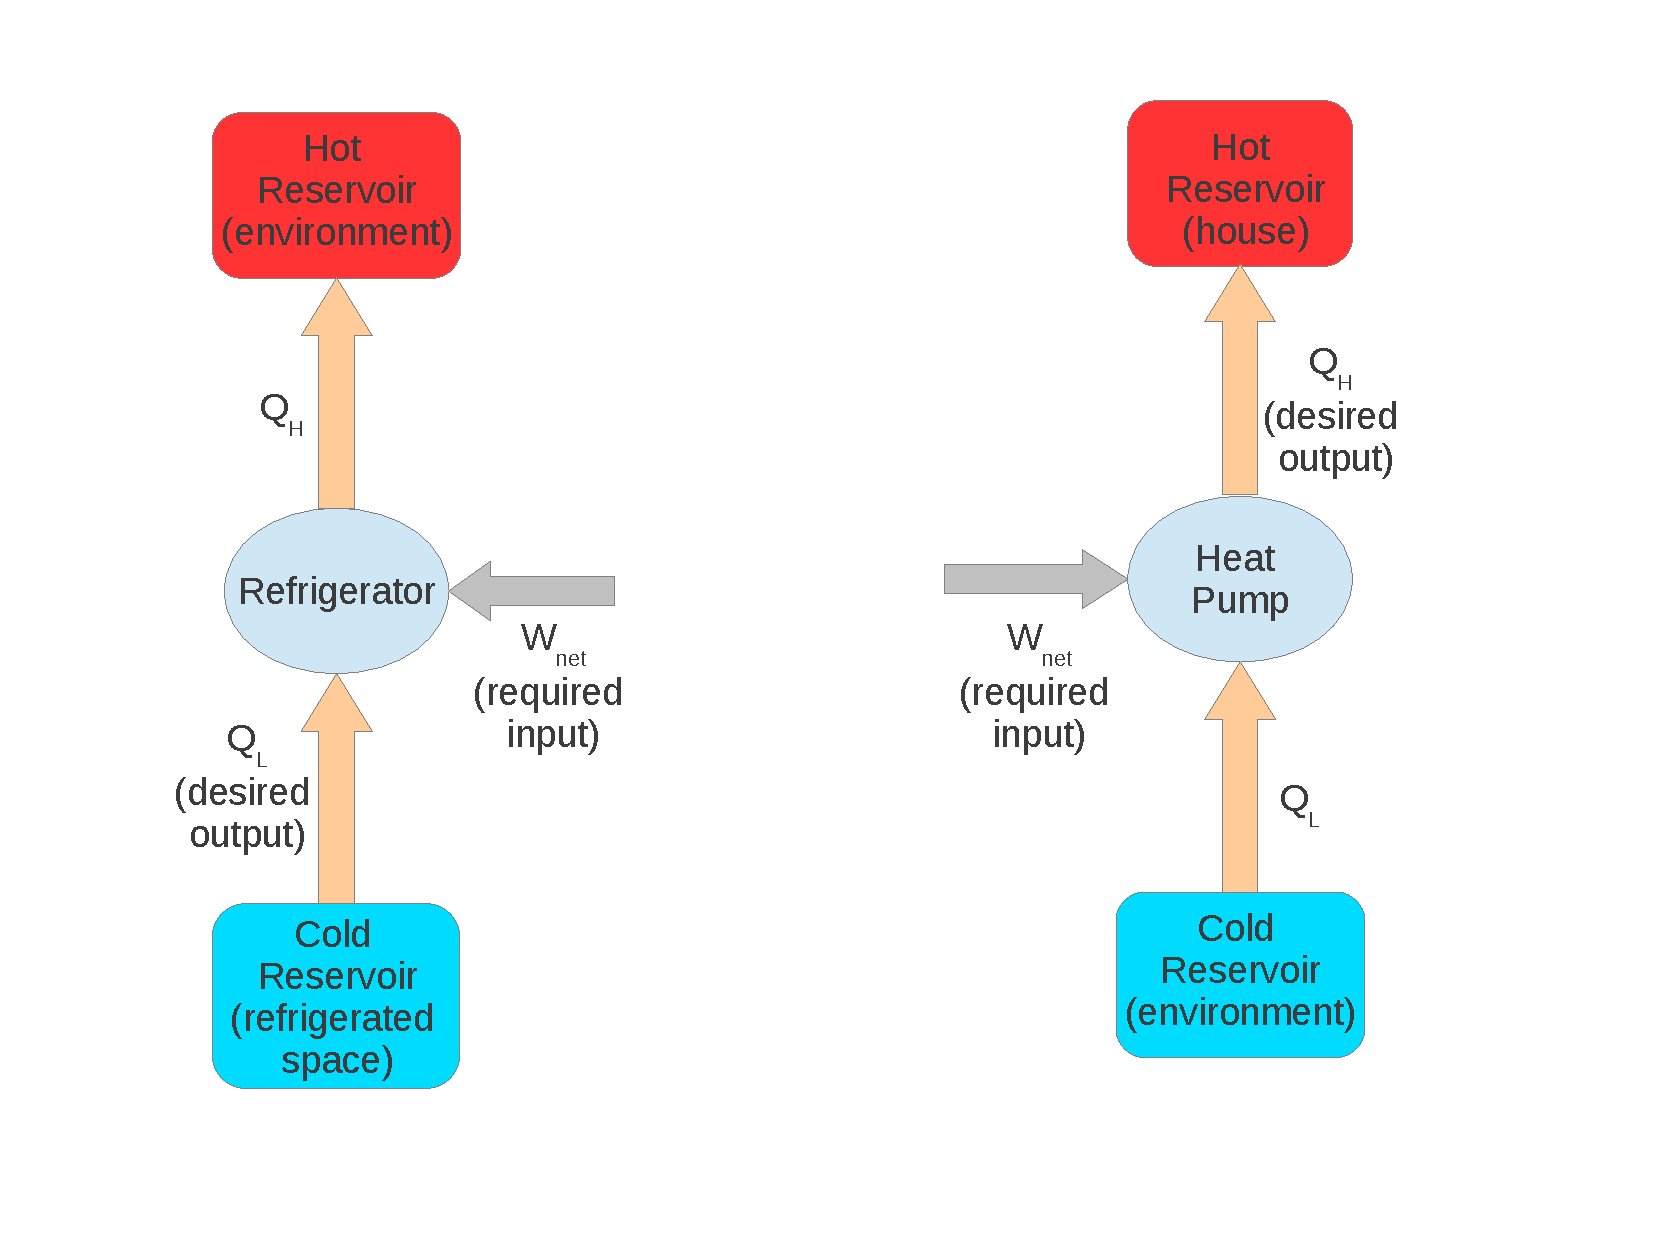
\includegraphics[width=7.5cm,clip]{./Pics/Overview_Refrig2}
     \end{center}
    \end{figure}
   \end{column}  
  \end{columns}
\end{frame}

%%%
%%% Slide
%%%
\begin{frame}
 \frametitle{Refrigerator and Heat Pump}
    \begin{figure}%
     \begin{center}
      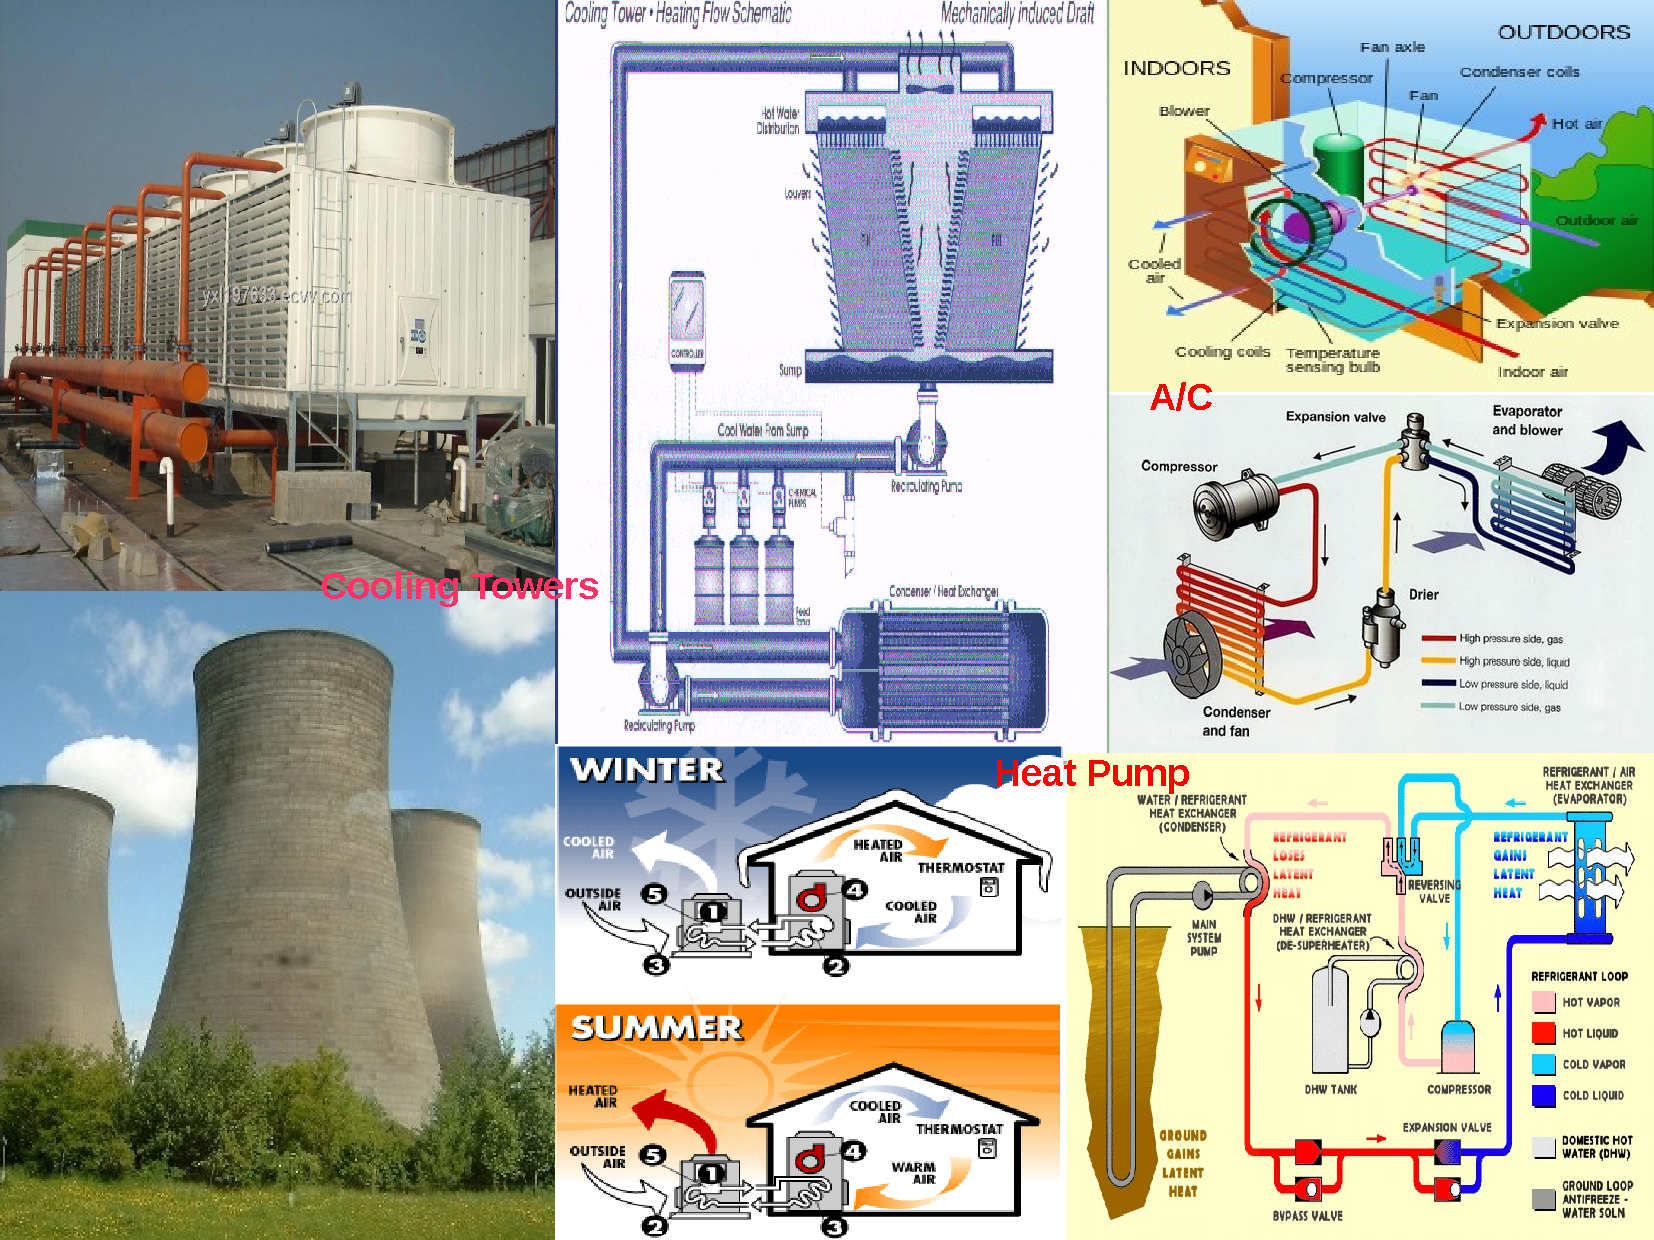
\includegraphics[width=12.cm,height=7.8cm]{./Pics/Overview_Refrig3}
     \end{center}
    \end{figure}
\end{frame}



%%%===            ===%%%
%%%=== SUBSECTION ===%%%
%%%===            ===%%%
\subsection{Assessing Refrigeration}
%%%
%%% Slide
%%%
\begin{frame}
 \frametitle{Coefficient of Performance (COP) and Unit of Refrigeration (Ton)}
    \begin{block}{\begin{center}\scriptsize Coefficient of Performance (COP)\end{center}}\scriptsize
        COP is the ratio of heat absorbed by the refrigerant while passing through the evaporator to the work input required to compress the refrigerant in the compressor, i.e., \blue{ratio between heat extracted and work done,}
        \visible<2->{\begin{equation}
            \text{COP}_{R} =\frc{\text{Desired Output}}{\text{Required Input}}=\frc{\text{Cooling Effect}}{\text{Work Input}}=\frc{Q_{L}}{W_{net,in}} = \frc{Q_{L}}{|Q_{H}|-Q_{L}}\label{Ref1:1}
        \end{equation}}
        \visible<3->{\begin{equation}
            \text{COP}_{HP} = \frc{\text{Desired Output}}{\text{Required Input}}=\frc{\text{Heating Effect}}{\text{Work Input}}=\frc{Q_{H}}{W_{net,in}} = \frc{Q_{H}}{|Q_{H}|-Q_{L}}    \label{Ref1:2}
       \end{equation}}
    \end{block}
     %\item <4-> In other words, it is the ratio between heat extracted and work done;
     %\item <4-> For fixed $Q_{L}$ and $Q_{H}$, Eqns. \ref{Ref1:1} and \ref{Ref1:2} lead to \textcolor{blue}{$\text{COP}_{HP}=\text{COP}_{R}+1$}.
     %\item <4->This means that \textcolor{blue}{COP$_{HP}>1$} (and also \textcolor{red}{COP$_{R}$) is positive}.
     \visible<4->{\begin{block}{\begin{center}\scriptsize Ton of Refrigeration\end{center}}\scriptsize
        \begin{enumerate}[(a)]\scriptsize
           \item<4-> \blue{Refrigeration effect} is the amount of heat extracted by the refrigerator from the refrigerated space;
           \item<4-> This effect is quantified by the \blue{unit of refrigeration} or \red{Ton of refrigeration};
           \item<4-> \red{One Ton (or Tonne)} of refrigeration is defined as the amount of heat removed from 1000 kg of water at 0$^{\text{o}}$C to form 1000 kg of ice within 24 hours. This quantifies the latent heat $\left(L_{f}\right)$ required to be removed for solidification of water at 0$^{\text{o}}$C, i.e.,
      \end{enumerate}
         \visible<5->{\begin{displaymath}
              \textcolor{red}{\text{1 Ton of Refrigeration}} = \text{mass of water} \times L_{f} = \text{ 12000 BTU/h} \sim \textcolor{blue}{210\;\; \text{kJ/min}} = \text{ 3.5 kW}\nonumber 
         \end{displaymath}}
     \end{block}}
 % \end{enumerate}
\end{frame}


%%%
%%% SECTION
%%%
\section{Reversed Carnot Cycle for Refrigeration}

%%%
%%% Slide
%%%
\begin{frame}
 \frametitle{Reversed Carnot Cycle}
  \begin{columns}
   \begin{column}[c]{0.45\linewidth}
    \begin{enumerate}[(1)]\scriptsize
      \item <1-> As we saw in Module 02, Carnot cycle (ideal) is the most efficient thermal cycle. It can also be used to get refrigerant effect upon its reversal;
      \item <1-> Refrigerated body needs to be kept at low temperature $T_{L}=T_{2}$ for which heat $\left(Q_{L}\right)$ should be removed at constant rate;
      \item <1-> Rejected to surroundings at high temperature, $T_{H}=T_{1}$;
      \item <1-> The amount of heat rejected to the surroundings is Q$_{H}$ while the net work done is {\it W};
      \item <1->The four stages are:
        \begin{enumerate}[(a)]\scriptsize
          \item<2-> 1-2: Reversible adiabatic compression;
          \item<2-> 2-3: Reversible isothermal heat rejection $\left(Q_{H}\right)$ at $T_{1}$;
          \item<2-> 3-4: Reversible adiabatic expansion;
          \item<2-> 4-1: Reversible isothermal heat absorption $\left(Q_{L}\right)$ at $T_{2}$;
        \end{enumerate}
     \end{enumerate}
   \end{column}
   \begin{column}[c]{0.55\linewidth}
    \begin{figure}%
     \begin{center}
      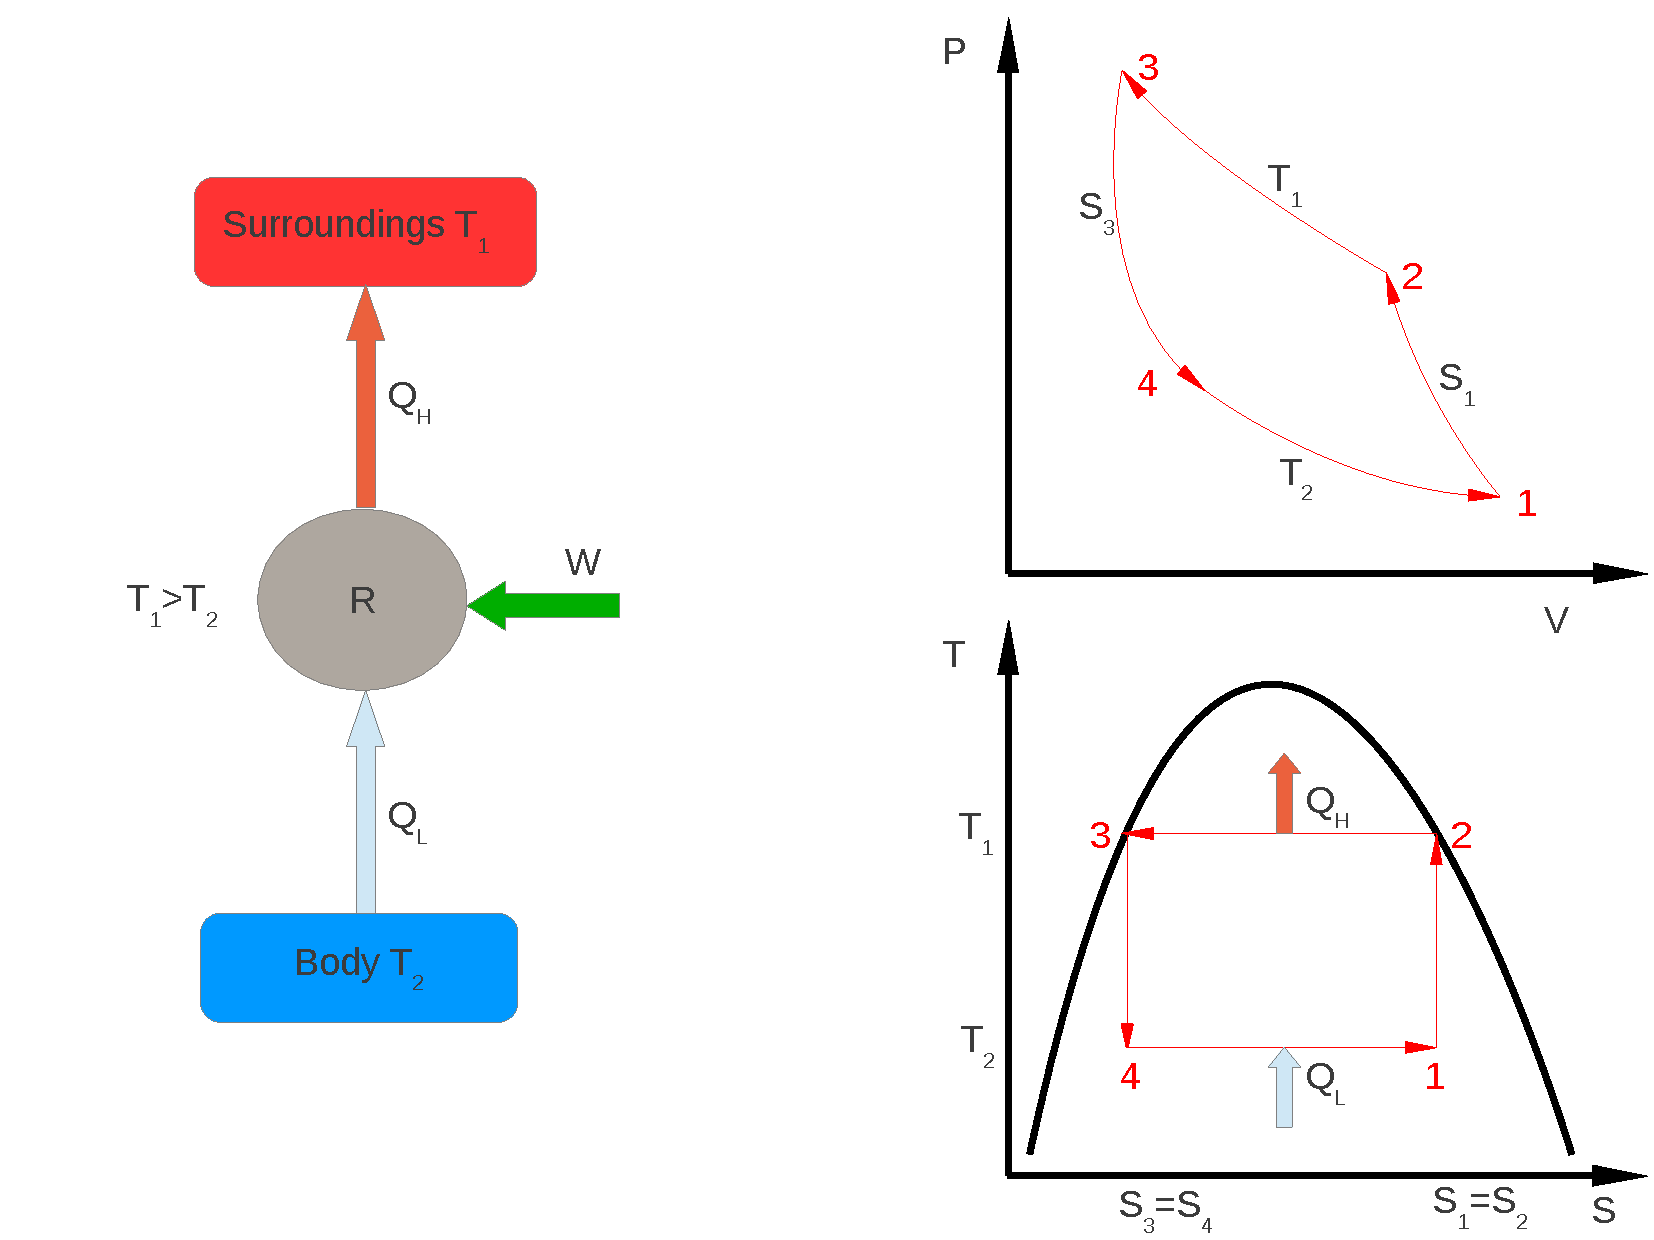
\includegraphics[width=6.8cm,height=6.5cm]{./Pics/Overview_Refrig4}
     \end{center}
    \end{figure}
   \end{column}   
  \end{columns}
\end{frame}
 

%%%
%%% Slide
%%%
\begin{frame}
 \frametitle{Reversed Carnot Cycle}
  \begin{columns}
   \begin{column}[c]{0.5\linewidth}
    \begin{enumerate}[(1)]\setcounter{enumi}{5}\scriptsize
      \item <1-> We should recall the Carnot thermal efficiency, $\eta_{T}=1-\frc{|Q_{L}|}{Q_{H}}$;
      \item <1-> Thus,
            \visible<1->{\begin{equation}\label{Refe1:3}
              \text{COP}_{HP}=\frc{1}{\eta_{T}}\;\;\;\text{ and }\;\;\;\text{COP}_{R}=\frc{1}{\eta_{T}}-1 
            \end{equation}}
      \item <2-> We can then conclude that the {\it COP} for any heat engine discussed in Module 02 operating on a reversed thermodynamic cycle (e.g., heat pump or refrigerator) could also be obtained from Eqn.~\ref{Refe1:3}.
      \item <3-> As the Carnot thermal efficiency can also be expressed as a function of the temperature of the hot and cold reservoirs, $\eta_{T}^{\text{Carnot}}=1-\frc{T_{L}}{T_{H}}=\frc{T_{H}-T_{L}}{T_{L}}$, the {\it COP} for Carnot engine running backwards can also be expressed as,
     \end{enumerate}
   \end{column}
   \begin{column}[c]{0.5\linewidth}
    \begin{figure}%
     \begin{center}
      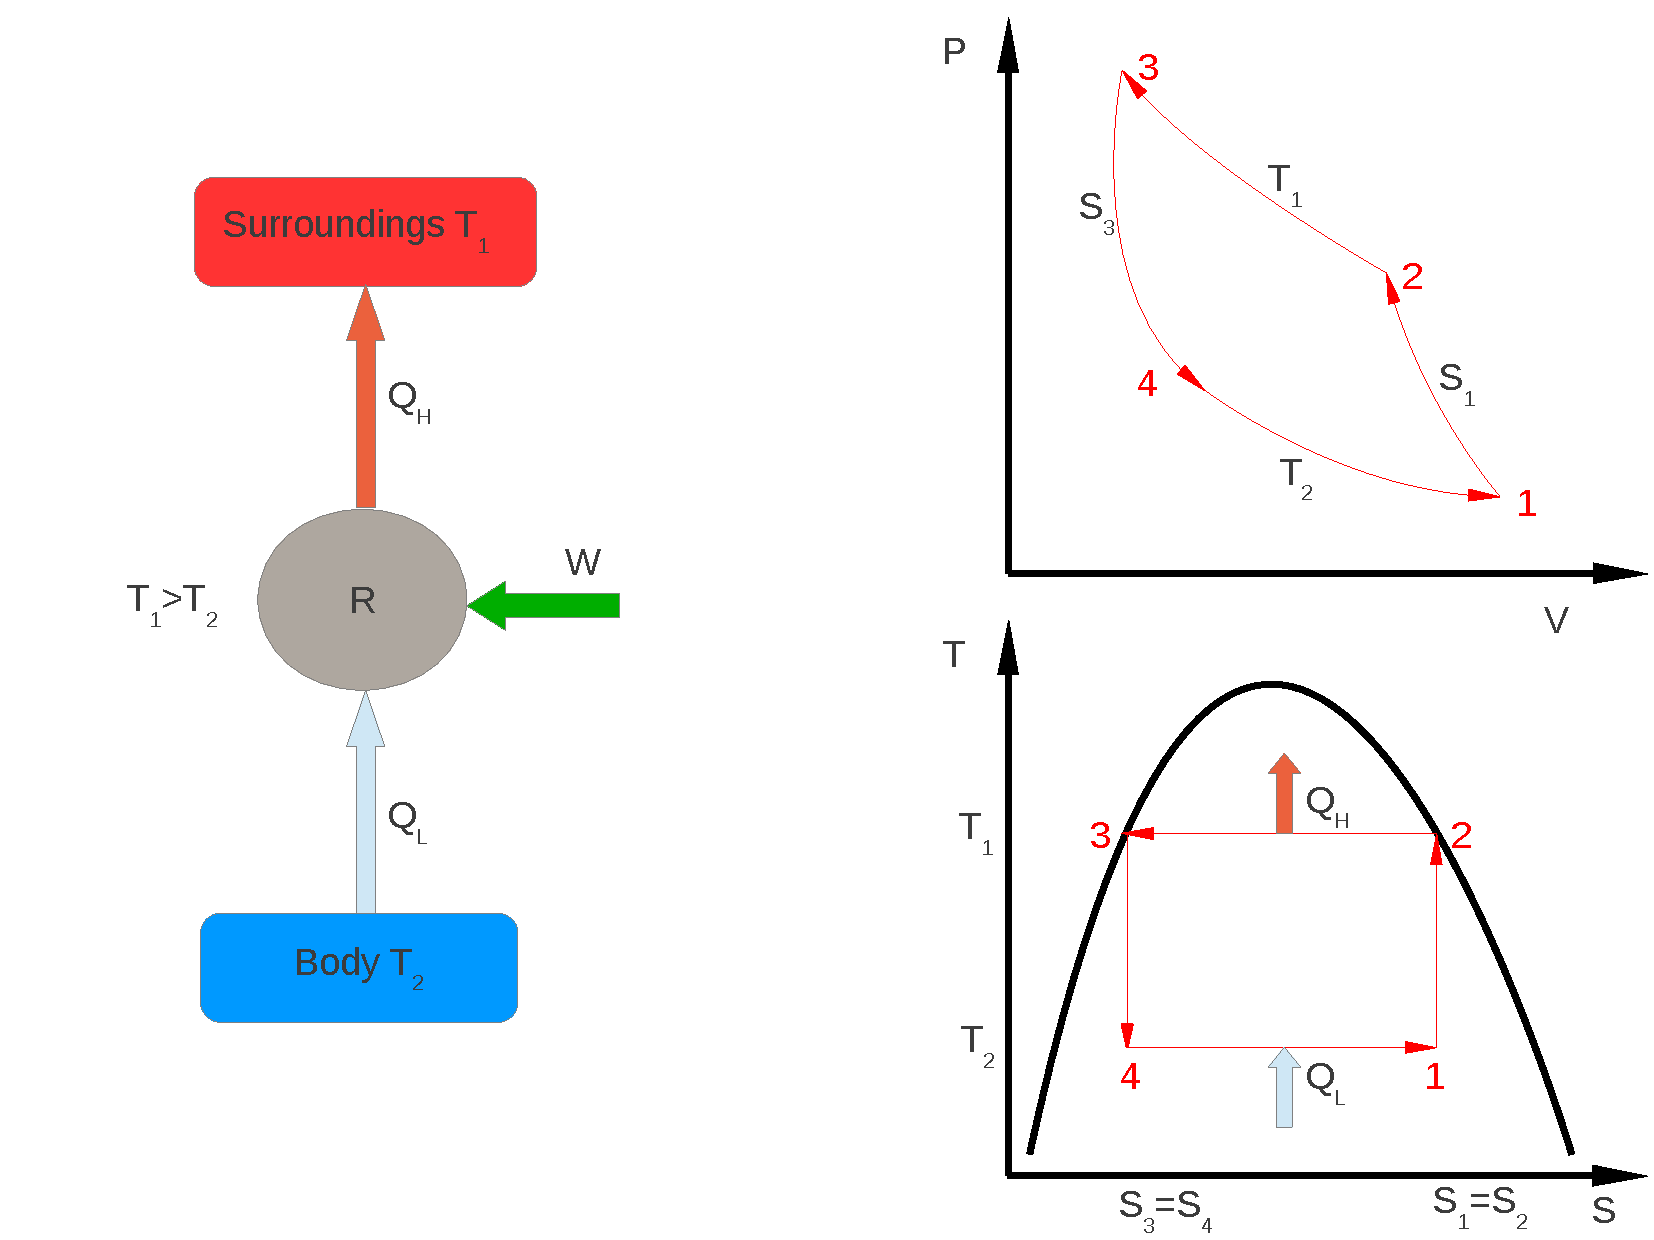
\includegraphics[width=6.cm,height=6.cm]{./Pics/Overview_Refrig4}
     \end{center}
    \end{figure}  
   \end{column}   
  \end{columns}

       \visible<3->{\begin{equation}\scriptsize
          \text{COP}_{HP}^{\text{Carnot}}=\frc{T_{H}}{T_{H}-T_{L}}\;\;\;\text{ and }\;\;\; \text{COP}_{R}^{\text{Carnot}}=\frc{T_{L}}{T_{H}-T_{L}}
       \end{equation}}
\end{frame}

%%%
%%% Slide
%%%
\begin{frame}
 \frametitle{Example 1: Reversed Carnot Cycle -- Heat Pump (Problem 1)}
    For the heating of a residence in a cold enviroment (-5$^{\text{o}}$C), a heat pump was used. The engine was designed to maintain the house's interior temperature at 25$^{\text{o}}$C. The compressor heat pump is driven by a heat engine working between 1000$^{\text{o}}$C and 25$^{\text{o}}$C. Assume that both cycles are reversibles, determine the ratio in which the heat pump and the heat engine share the heating load.

 
\end{frame}


%%%
%%% SECTION
%%%
\section{Gas Refrigeration}


%%%

%%%===            ===%%%
%%%=== SUBSECTION ===%%%
%%%===            ===%%%
\subsection{Air Standard Gas-Refrigeration Cycles}

%%% Slide
%%%
\begin{frame}
 \frametitle{Air Standard Cycle}
The following assumptions are usually applied to gas-refrigeration air-standard cycles analysis:
  \begin{enumerate}[(a)]
   \item <2-> The working fluid is a fixed mass of air that behaves as an ideal gas;
   \item <2-> All inlet and exhaust processes in open-loop systems are replaced by heat transfer processes to or from the environment;
   \item <3-> \blue{All processes within the cycle are reversible};
   \item <3-> \blue{The air has constant specific heat capacities};
   \item <3-> MW = 29 g.mol$^{-1}$, C$_{p}$ = 1.005 kJ.(kg.K)$^{-1}$ and C$_{v}$ = 0.718 kJ.(kg.K)$^{-1}$, where MW is the molar mass and C$_{p}$ and C$_{v}$ are the heat capacities at constant pressure and volume, respectively.
  \end{enumerate}
\end{frame}


%%%===            ===%%%
%%%=== SUBSECTION ===%%%
%%%===            ===%%%
\subsection{Reversed Brayton Cycle}

%%%
%%% Slide
%%%
\begin{frame}
 \frametitle{Bell-Coleman Cycle (or Reversed Brayton Cycle)}
    \begin{columns}
       \begin{column}[c]{0.55\linewidth}
          \begin{figure}%
            \begin{center}
               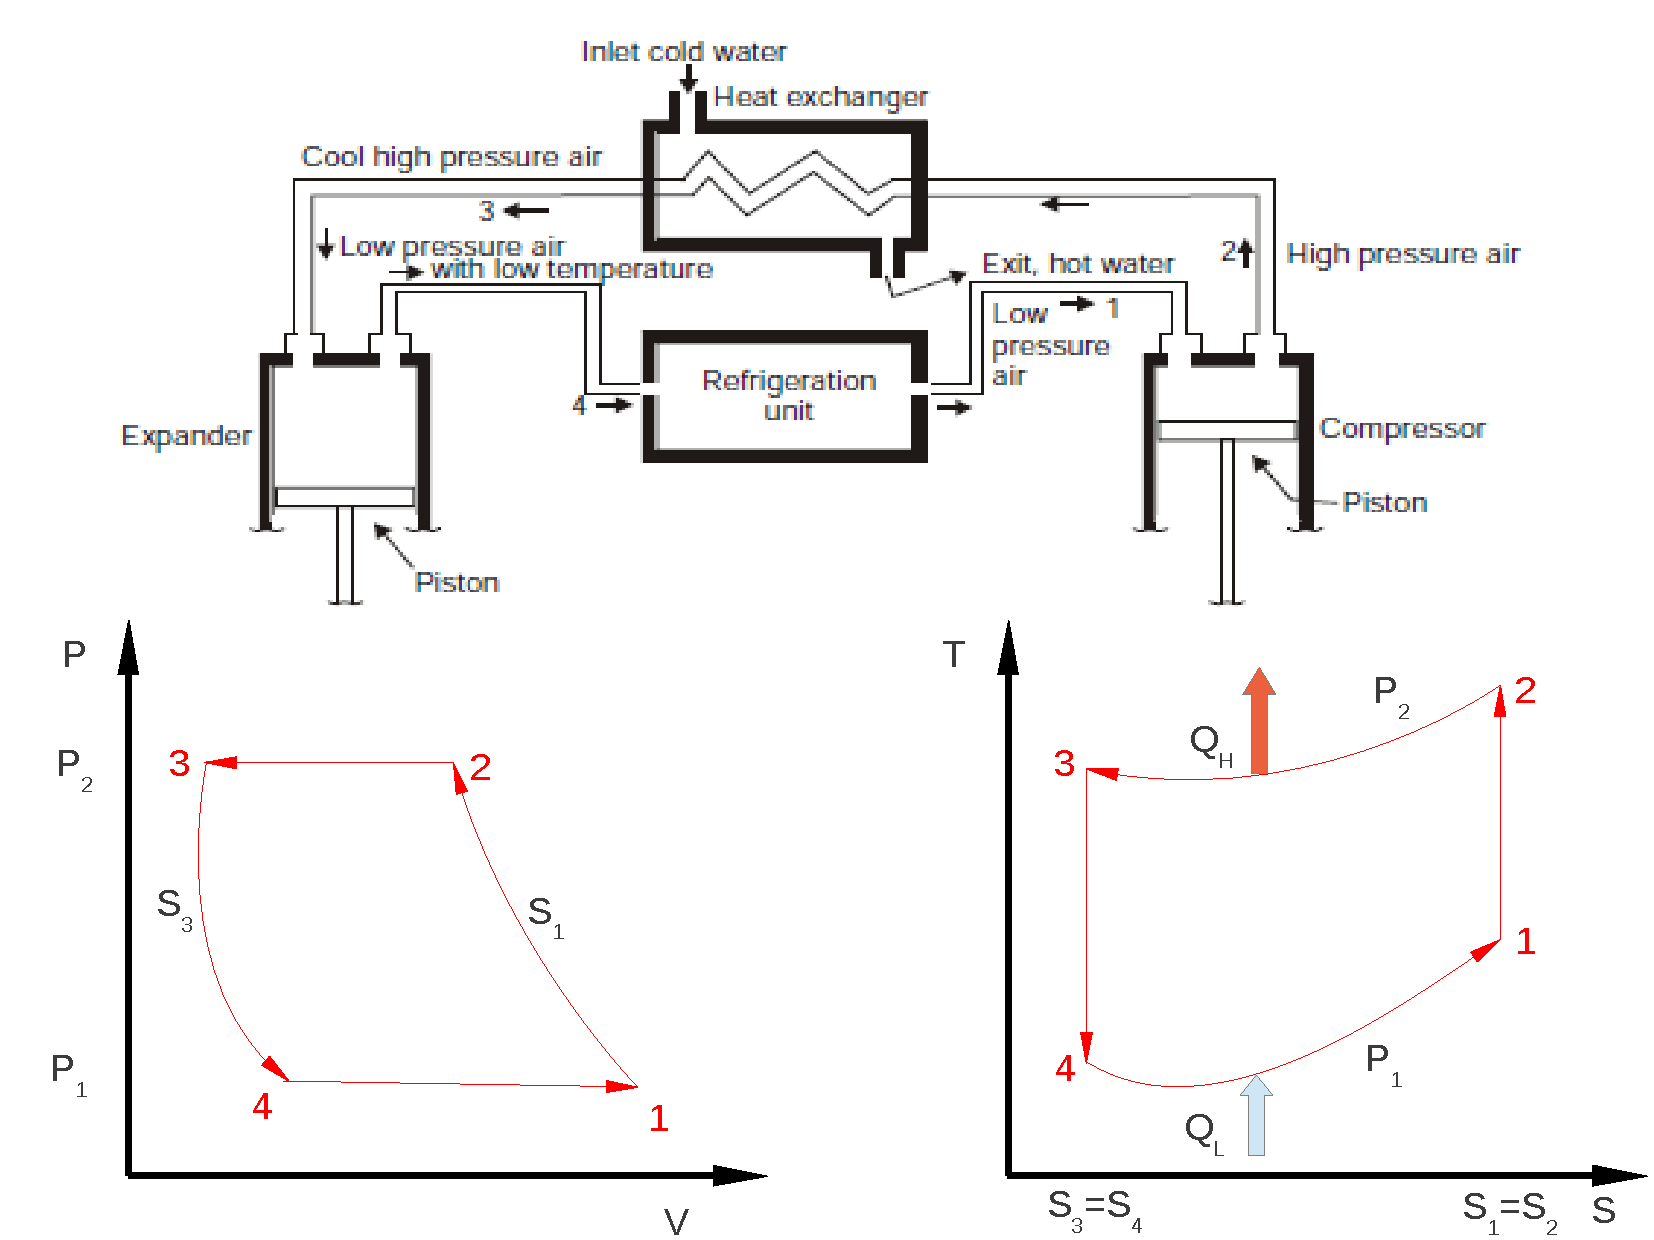
\includegraphics[width=\columnwidth]{./Pics/Overview_Refrig6}
            \end{center}
          \end{figure}  
       \end{column}
       \begin{column}[c]{0.45\linewidth}
         \begin{enumerate}[(1)]\scriptsize
           \item <1-> Bell-Coleman Cycle uses air as a refrigerant and is a modified form of the reversed Carnot cycle where;
           \item <1-> Isothermal heat addition and release are replaced by isobaric processes;   
           \item <2-> Mostly used in cargo ships and aircraft refrigeration;
           \item <3-> The process involves compressor, heat exchanger, expander and refrigeration unit.
         \end{enumerate}
      \end{column}
   \end{columns} 
\end{frame}

%%%
%%% Slide
%%%
\begin{frame}
 \frametitle{Bell-Coleman Cycle (or Reversed Brayton Cycle)}
  \begin{columns}

   \begin{column}[c]{0.6\linewidth}
    \begin{figure}%
     \begin{center}
      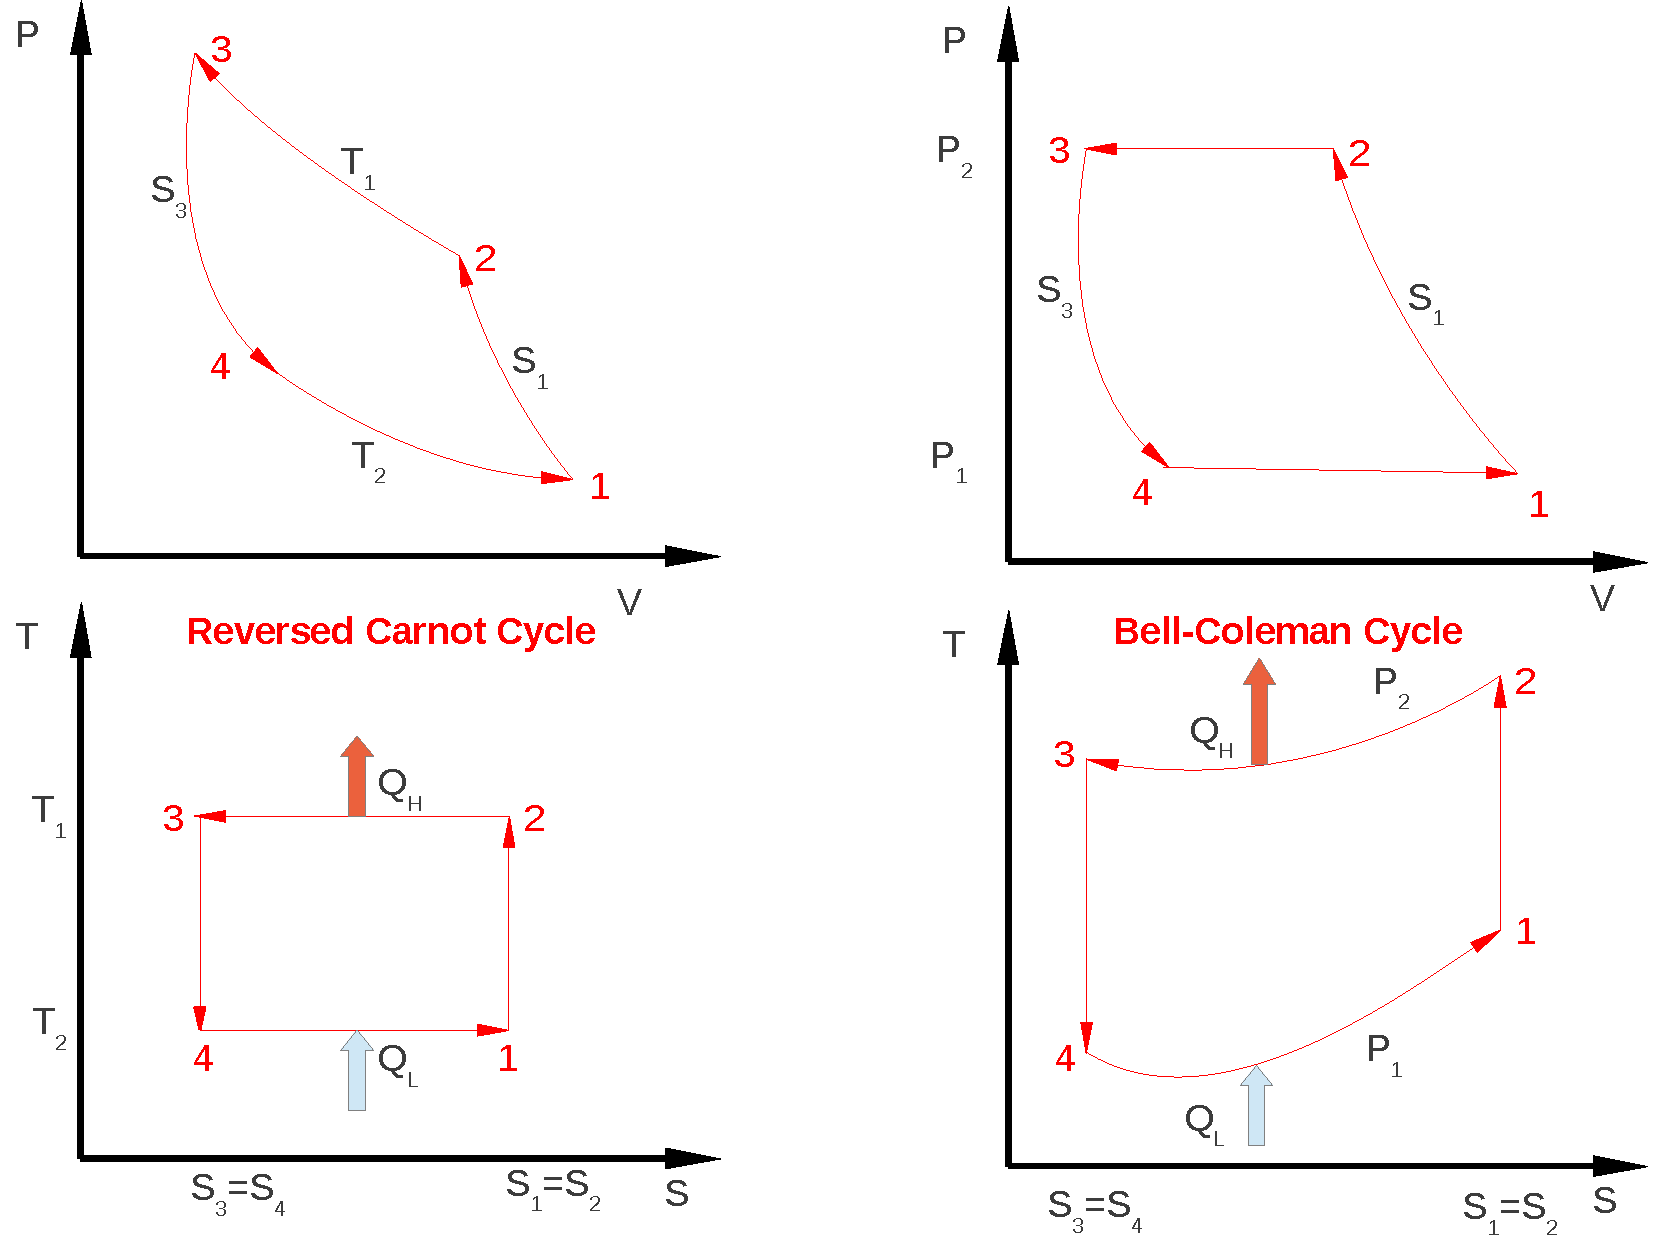
\includegraphics[width=\columnwidth]{./Pics/Overview_Refrig7}
     \end{center}
    \end{figure}  
   \end{column}  

   \begin{column}[c]{0.4\linewidth} 
      \begin{enumerate}[(1)]\setcounter{enumi}{4}\scriptsize
         \item <2-> 1-2: Adiabatic compression of air;
         \item <3-> 2-3: Isobaric heat rejection:
           \visible<3->{\begin{equation}
              Q_{\text{rejected}}=mC_{p}\left(T_{2}-T_{3}\right)
           \end{equation}}
         \item <4-> 3-4: Adiabatic expansion;
         \item <5-> 4-1: Isobaric heat absorption:
          \visible<5->{\begin{equation}
             Q_{\text{absorbed}}=mC_{p}\left(T_{1}-T_{4}\right)
          \end{equation}}
      \end{enumerate}
   \end{column}
  \end{columns}

\end{frame}


%%%
%%% Slide
%%%
\begin{frame}
 \frametitle{Thermodynamic Analysis}
    \begin{enumerate}[(1)]\setcounter{enumi}{8}\scriptsize
     \item <1-> The net work done upon system,
       \visible<1->{\begin{eqnarray}
          W &=& \left(\text{Heat Rejected - Heat Absorbed}\right) \nonumber \\
            &=& mC_{p}\left(T_{2}-T_{3}\right) - mC_{p}\left(T_{1}-T_{4}\right)
       \end{eqnarray}}
     \item <2-> Last lecture we defined the Coefficient of Performance as,
       \visible<2->{\begin{eqnarray}
          \textcolor{blue}{\text{COP}} &=& \frc{\text{Desired Effect}}{\text{Net Work}} = \frc{mC_{p}\left(T_{1}-T_{4}\right)}{mC_{p}\left(T_{2}-T_{3}\right) - mC_{p}\left(T_{1}-T_{4}\right)} \nonumber \\
                  &=& \textcolor{blue}{\frc{1}{\left(\frc{T_{2}}{T_{1}}-\frc{T_{3}}{T_{4}}\right)-1}} \label{refrig_CopIdeal}
        \end{eqnarray}}
     %\item <3-> Equation \ref{refrig_CopIdeal} describes the COP for \textcolor{blue}{ideal processes}. 
    \end{enumerate}
\end{frame}


%%%
%%% Slide
%%%
\begin{frame}
 \frametitle{Example 2: Bell-Coleman Cycle (Reversed Brayton Cycle, Problem 2)}\scriptsize
 A refrigerating engine operates on the Bell-Coleman cycle (of 6 tonnes capacity) with upper limiting pressure of 5.2 bar. Pressure and temperature at the beginning of the compression stage are 1.0 bar and 16$^{\text{o}}$C, respectively. The compressed air is cooled at constant pressure from a temperature of 41$^{\text{o}}$C  (flow entering the expansion cylinder). Assuming that both expansion and compression processes are adiabatic with $\gamma=1.4$ and the latent heat of fusion of water $\left(\text{L}_{\text{f}}\right)$ is 336 kJ/kg determine:

\begin{enumerate}[(a)]\scriptsize
\item COP;
\item Mass flow rate of air in circulation (kg/min);
\item Piston displacement of compressor and expander;
\item Bore of compressor and expansion cylinders. The unit runs at 240 rpm. Assume that the stroke length is 200 mm;
\item Power required to drive the unit.
\end{enumerate}

\end{frame}

%%%
%%% SECTION
%%%
\section{Vapour-Compression Refrigeration Cycle}

%%%===            ===%%%
%%%=== SUBSECTION ===%%%
%%%===            ===%%%
\subsection{Introduction}

%%%
%%% Slide
%%%
\begin{frame}
 \frametitle{Introduction}

  \scriptsize A few animations for reversed Brayton, Rankine cycles can be found in:
\href{http://www.sfsb.unios.hr/test/testhome/vtAnimations/animations/chapter09/refrigeration/index1.html}{\scriptsize{http://www.sfsb.unios.hr/test/testhome/vtAnimations/animations/chapter09/refrigeration/index1.html}}


  \begin{columns}
   \begin{column}[c]{0.45\linewidth}
    \begin{figure}%
     \begin{center}
      \visible<2->{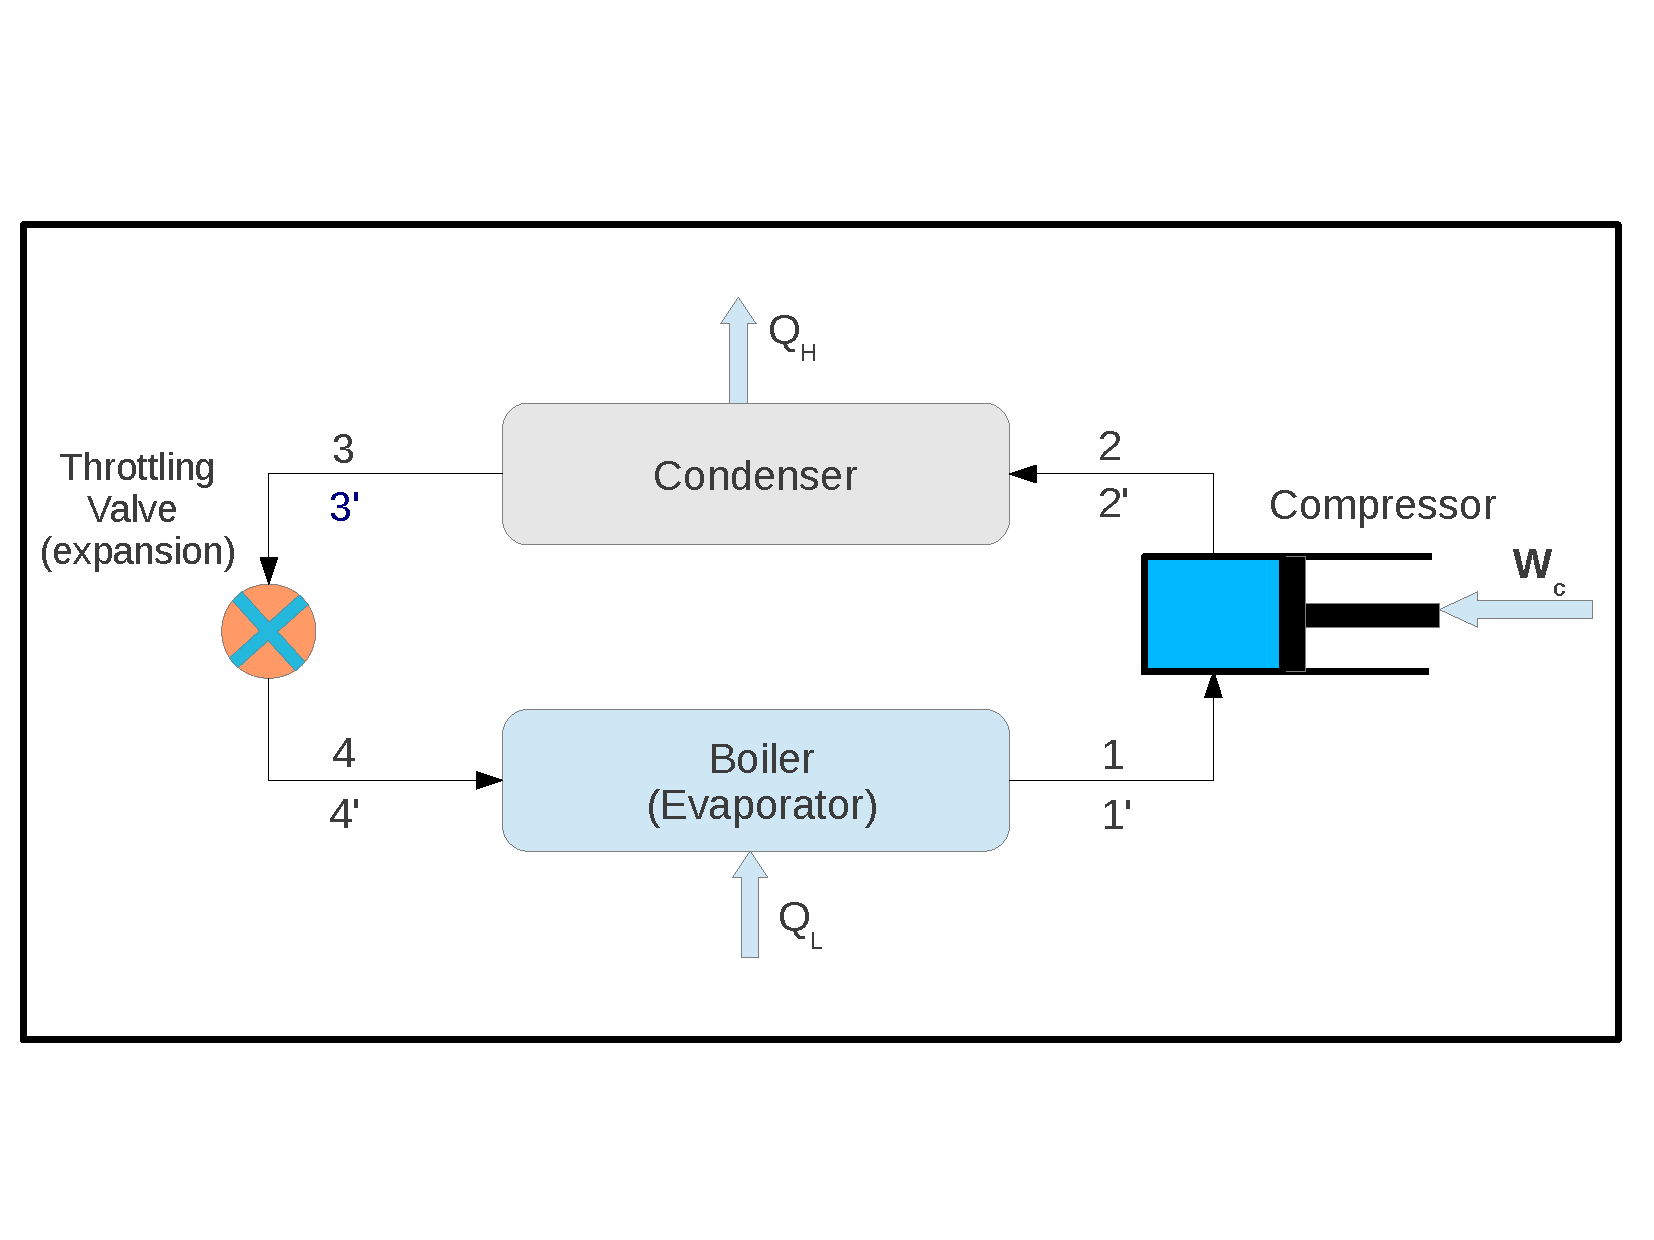
\includegraphics[width=\columnwidth,clip]{./Pics/Overview_Refrig12}}
     \end{center}
    \end{figure}  
   \end{column}  
   \begin{column}[c]{0.55\linewidth}
  \begin{enumerate}[(1)]\scriptsize
   \item <2-> First vapour-compression refrigeration system was a closed system introduced by Jacob Perkins (1766-1849) using \textcolor{blue}{diethyl ether} as refrigerant fluid;
   \item <2-> Ether vapour was compressed in a piston-cylinder system and condensed (i.e., turned into liquid) at a higher saturation pressure and temperature;
   \item <2-> Liquid ether is throttled through a valve back into the low-pressure evaporator;
   \item <2-> This process takes place beneath the vapour dome of the ether and it is a \textcolor{blue}{reversed Rankine cycle}.
   \item <3-> In most industrial applications, vapour compression systems occur in closed cycles.
  \end{enumerate}
 \end{column}  
\end{columns}

\end{frame}

%%%===            ===%%%
%%%=== SUBSECTION ===%%%
%%%===            ===%%%
\subsection{Dry and Wet Compression Refrigeration Cycles}

%%%
%%% Slide
%%%
\begin{frame}
 \frametitle{Dry Compression Cycle} 
  \begin{columns}
   \begin{column}[c]{0.5\linewidth}
    \begin{figure}%
     \vbox{
      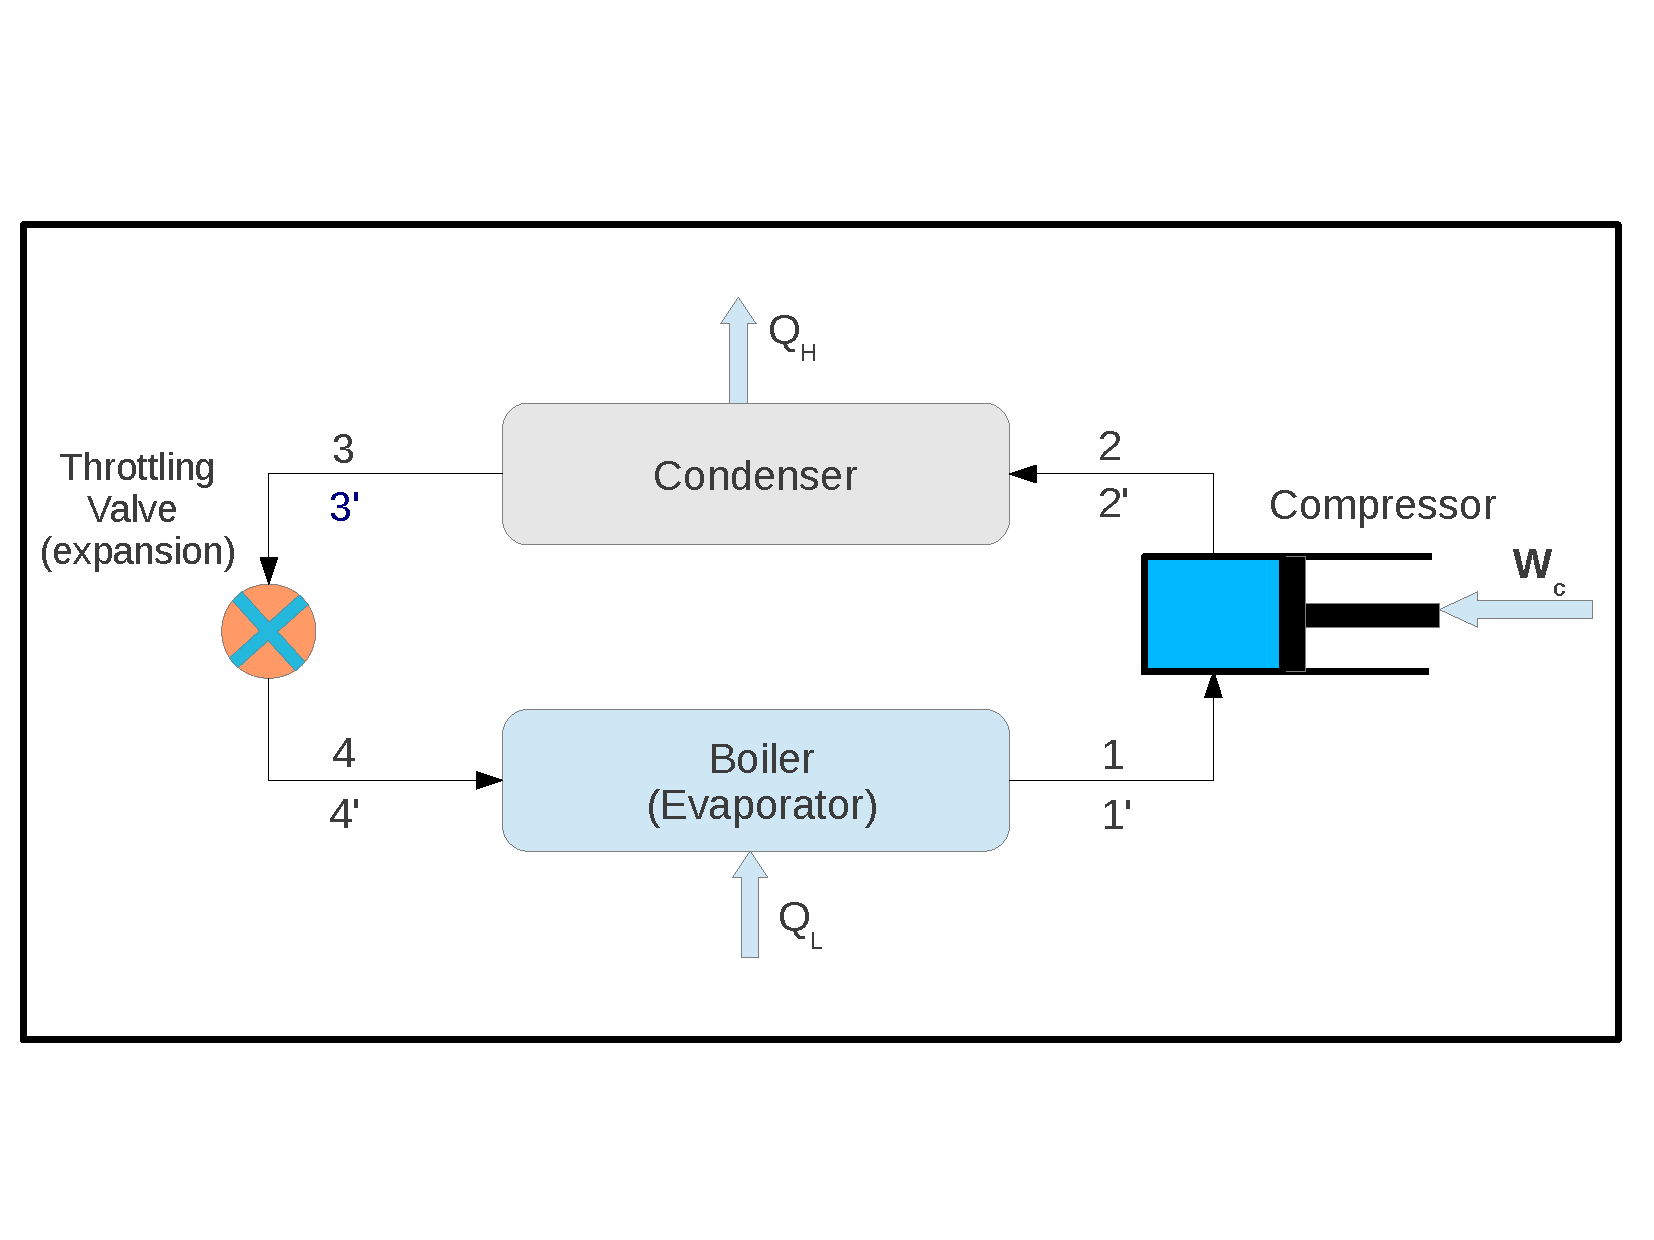
\includegraphics[width=5.5cm,clip]{./Pics/Overview_Refrig12}
      \vspace{-.5cm}
      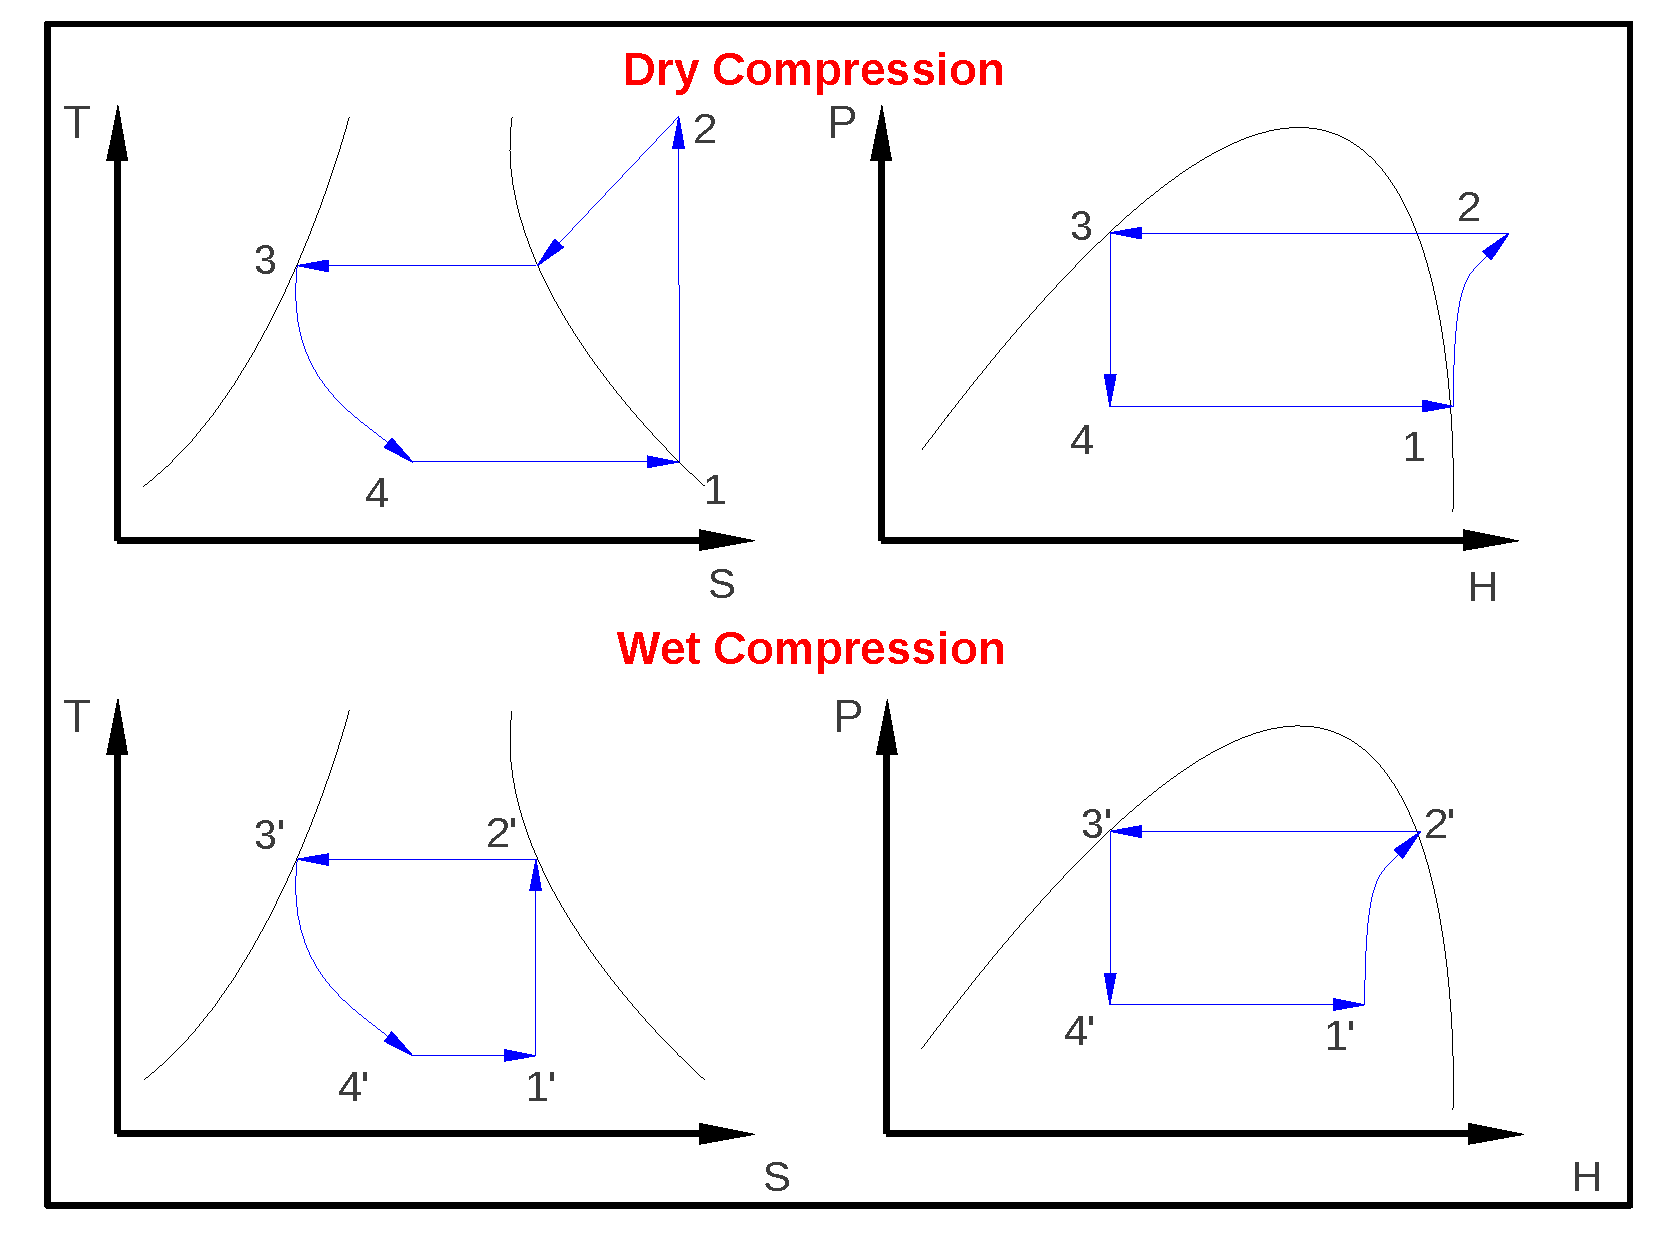
\includegraphics[width=4.5cm,clip]{./Pics/Overview_Refrig13}}
    \end{figure}  
   \end{column}  
   \begin{column}[c]{0.5\linewidth}
  \begin{enumerate}[(1)] \scriptsize
   \item <1-> Refrigerant (in gas/vapour phase) is compressed isentropically in \textcolor{blue}{compressor from state 1 to 2}; 
   \item <1-> \textcolor{blue}{High pressure and high temperature} fluid enters the condenser at \textcolor{blue}{state 2};
   \item <1-> The condensed fluid (saturated liquid at high pressure, state 3) is driven into the expansion valve where an \textcolor{blue}{isenthalpic expansion} occurs.
   \item <1-> The refrigerant fluid leaves the expansion valve (state 4) as a \textcolor{blue}{low pressure wet mixture of liquid and vapour};
   \item <2-> This mixture is driven into the evaporator where heat is transferred from the surroundings and thereby showing refrigerant effect; 
   \item <2-> Due to this \textcolor{blue}{heat absorption}, the liquid-vapour mixture is transformed into a \textcolor{red}{dry gaseous refrigerant} and;
   \item <3-> This process is called \textcolor{blue}{Dry Compression} in which,
   \item <3-> The compression of this dry refrigerant yields \textcolor{blue}{superheated state} of the fluid as shown in \textcolor{blue}{state 2}.
  \end{enumerate}
 \end{column}  
\end{columns}
\end{frame}


%%%
%%% Slide
%%%
\begin{frame}
 \frametitle{Wet Compression Cycle} 
  \begin{columns}
   \begin{column}[c]{0.5\linewidth}
    \begin{figure}%
     \vbox{
      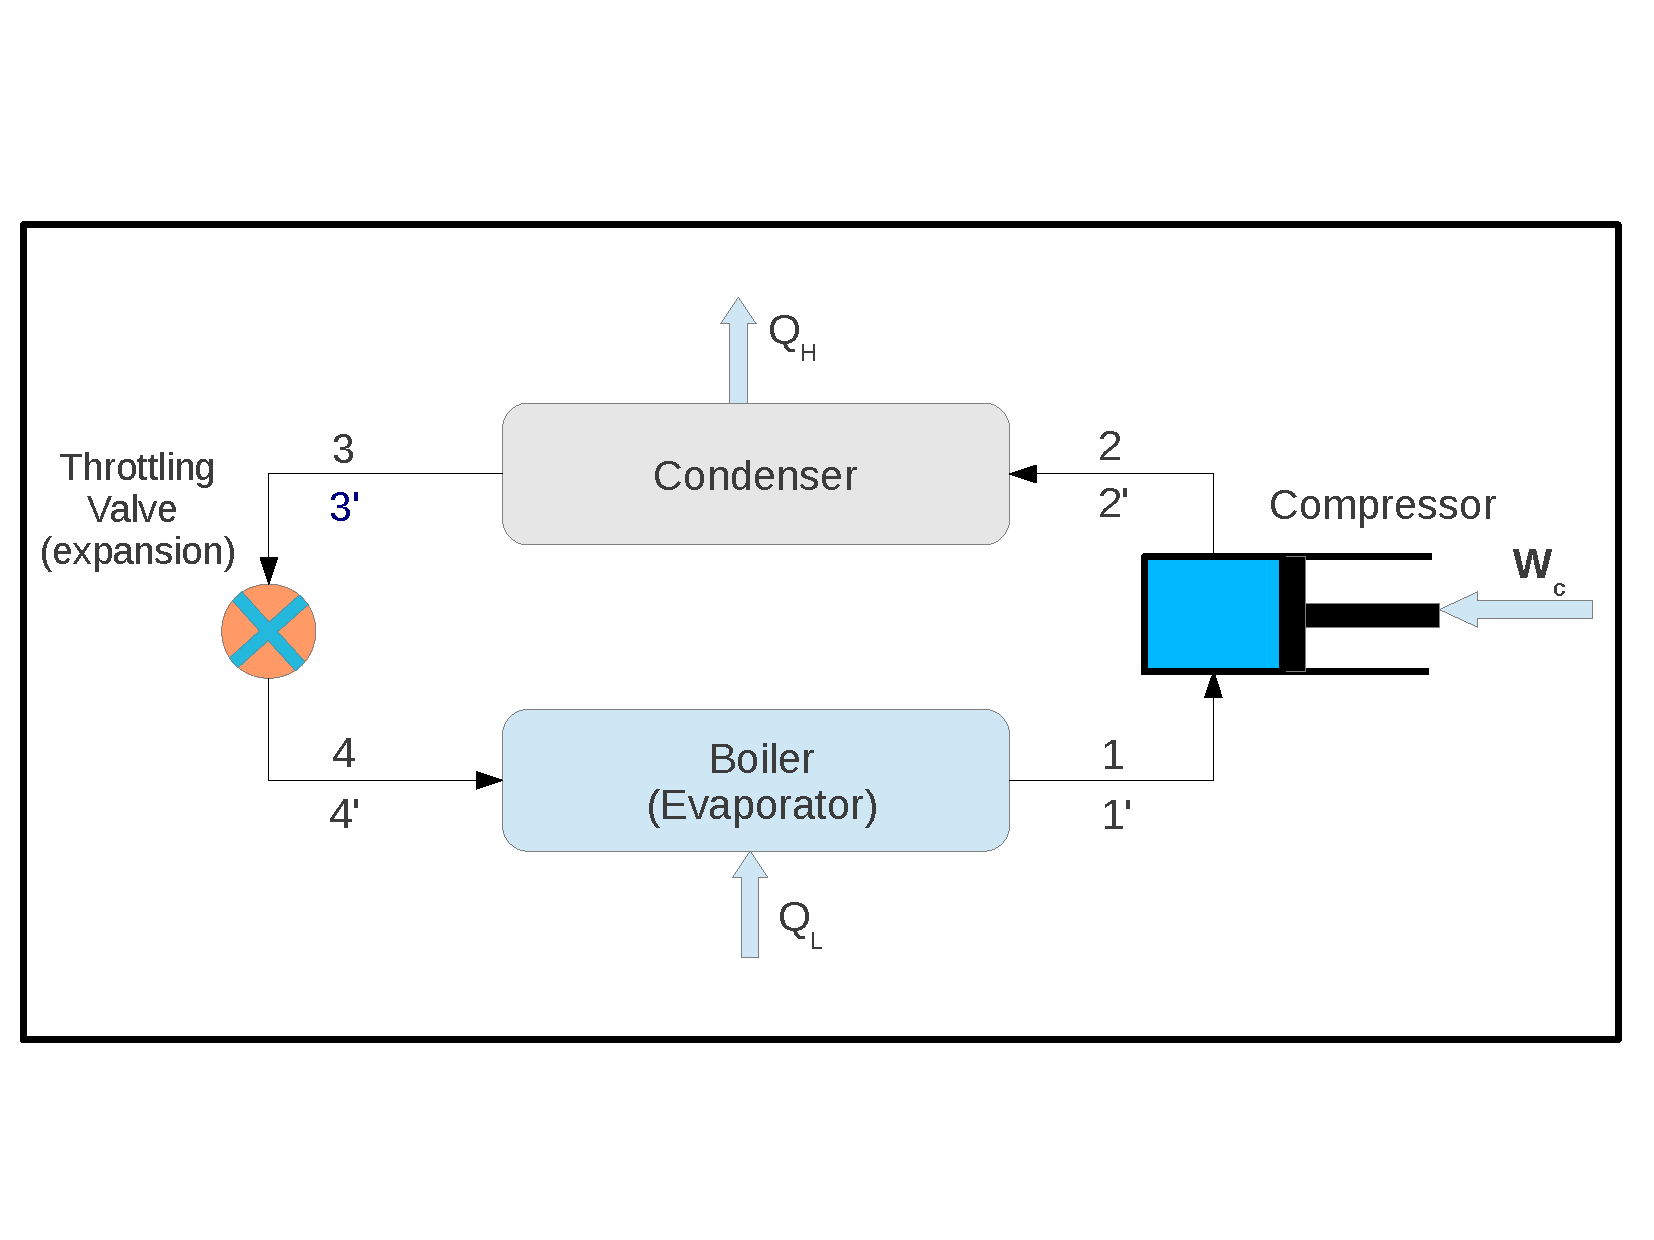
\includegraphics[width=5.5cm,clip]{./Pics/Overview_Refrig12}
      \vspace{-.5cm}
      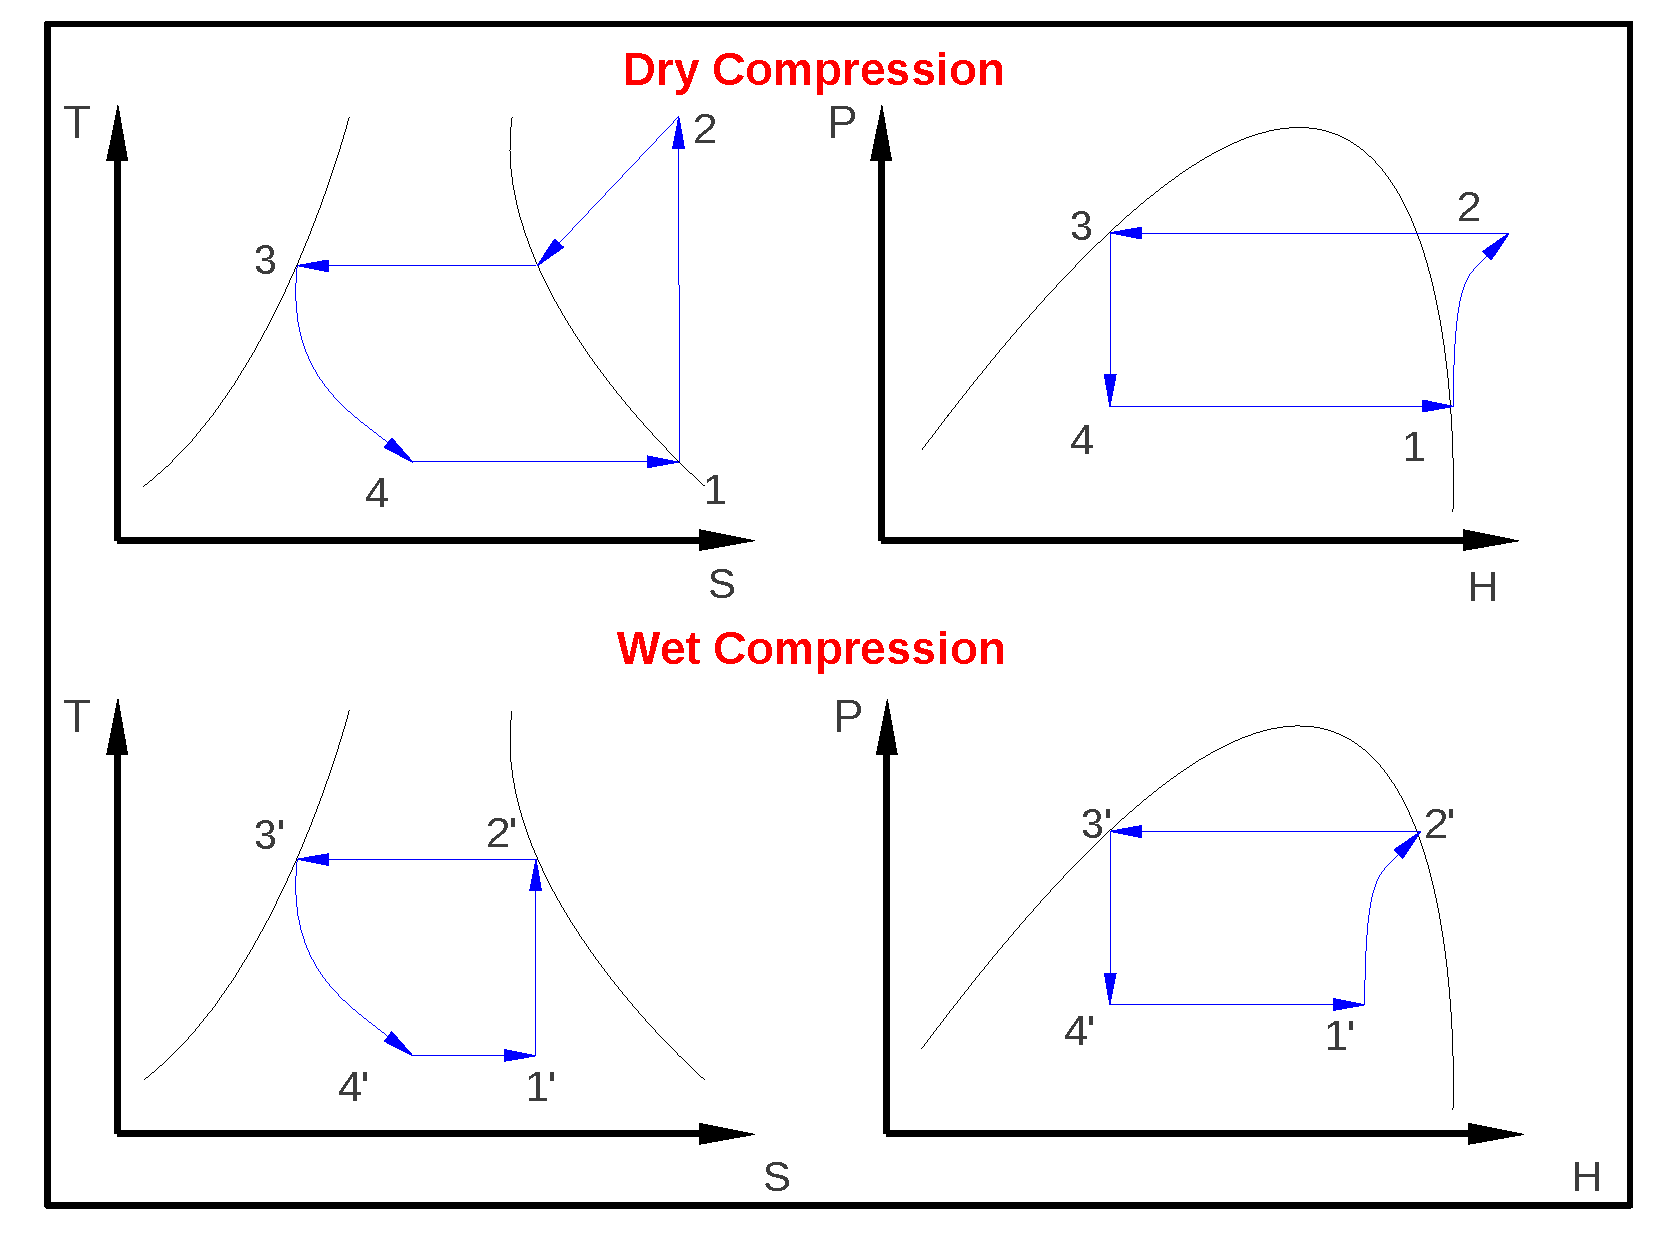
\includegraphics[width=4.5cm,clip]{./Pics/Overview_Refrig13}}
    \end{figure}  
   \end{column}  
   \begin{column}[c]{0.5\linewidth}
  \begin{enumerate}[(1)] \setcounter{enumi}{8}\scriptsize
     \item <1-> In this case, the \textcolor{blue}{liquid-vapour mixture (state 1$^{\prime}$)} is injected in the compressor;
     \item <1-> In the compressor, the wet mixture is transformed into a \textcolor{blue}{dry refrigerant fluid} (gas phase -- state 2$^{\prime}$);
     \item <1-> The dry refrigerant at \textcolor{blue}{high pressure and high temperature} is driven into the condenser where the fluid is turned into saturated liquid at high pressure;
     \item <1-> The refrigerant is throttled from high to low pressure inside the expansion valve (states 3$^{\prime}$-4$^{\prime}$);
     \item <1-> The refrigerant is then driven towards the evaporator (states 4$^{\prime}$ 1$^{\prime}$) where it absorbs heat from the surroundings and ;
     \item <1-> Part of the liquid fraction is evaporated \textcolor{red}{but it does not become dry (gas) refrigerant} at the inlet of the compressor.

  \end{enumerate}
 \end{column}  
\end{columns}
\end{frame}


%%%
%%% Slide
%%%
\begin{frame}
 \frametitle{Thermodynamic Analysis} 
  \begin{columns}
   \begin{column}[c]{0.6\linewidth}
     \begin{enumerate}[(1)]\scriptsize
       \item<1-> Four Stages:
         \begin{enumerate}[(a)]\scriptsize
            \item <1-> 1-2 or 1$^{\prime}$-2$^{\prime}$: isentropic compression;
            \item <1-> 2-3 or 2$^{\prime}$-3$^{\prime}$: isobaric heat rejection;
            \item <1-> 3-4 or 3$^{\prime}$-4$^{\prime}$: isenthalpic expansion ;%process or throttling process;
            \item <1-> 4-1 or 4$^{\prime}$-1$^{\prime}$: isobaric heat absorption.
         \end{enumerate}
       \item<2-> For a mass flow rate of refrigerant \blue{$\dot{m}$} (kg/s):
         \begin{enumerate}[(a)]\scriptsize
           \item<2-> The \blue{refrigeration capacity} (or refrigeration effect) is,\\
               \visible<2->{\begin{displaymath}
                Q_{\text{absorbed}}^{\text{(dry)}} = \dot{m}\left(h_{1}-h_{4}\right) \;\text{;}\; Q_{\text{absorbed}}^{\text{(wet)}} = \dot{m}\left(h_{1^{\prime}}-h_{4^{\prime}}\right)         
             \end{displaymath}}
           \item <3-> And the \blue{net work} (= work input) is,
             \visible<3->{\begin{displaymath}     
                W_{\text{compressor}}^{\text{(dry)}} = \dot{m}\left(h_{2}-h_{1}\right) \;\text{;}\; W_{\text{compressor}}^{\text{(wet)}} = \dot{m}\left(h_{2^{\prime}}-h_{1^{\prime}}\right) 
             \end{displaymath}}
           \item<4-> And the \blue{Coefficient of Performance (COP)} is,
             \visible<4->{\begin{eqnarray}
                && COP^{\text{(dry)}} = \frc{\text{Refrigeranting Capacity}}{\text{Work done}} = \frc{h_{1}-h_{4}}{h_{2}-h_{1}}   \nonumber \\ 
                && COP^{\text{(wet)}} = \frc{h_{1^{\prime}}-h_{4^{\prime}}}{h_{2^{\prime}}-h_{1^{\prime}}} \nonumber
             \end{eqnarray}}
         \end{enumerate}
     \end{enumerate}
   \end{column}  
   \begin{column}[c]{0.4\linewidth}
     \vbox{
      \hbox{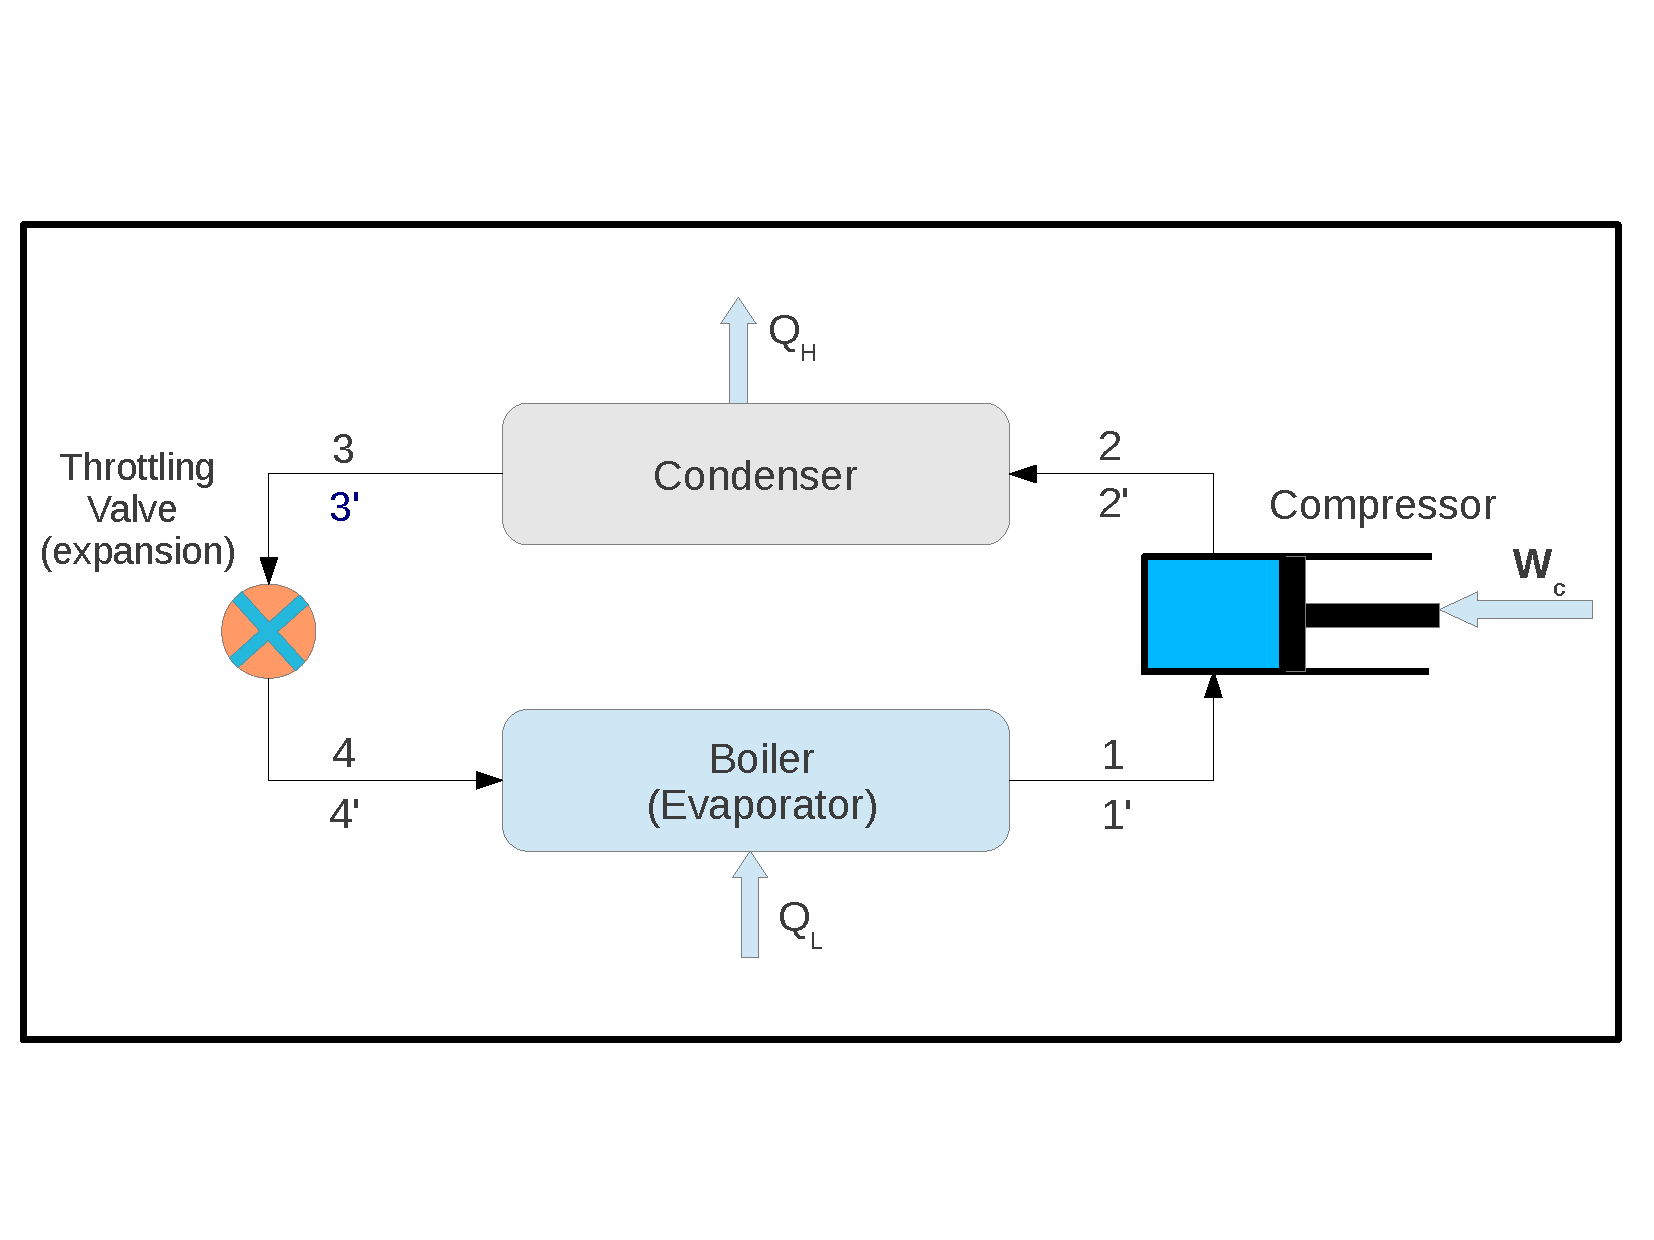
\includegraphics[width=.9\columnwidth]{./Pics/Overview_Refrig12}}
      \hbox{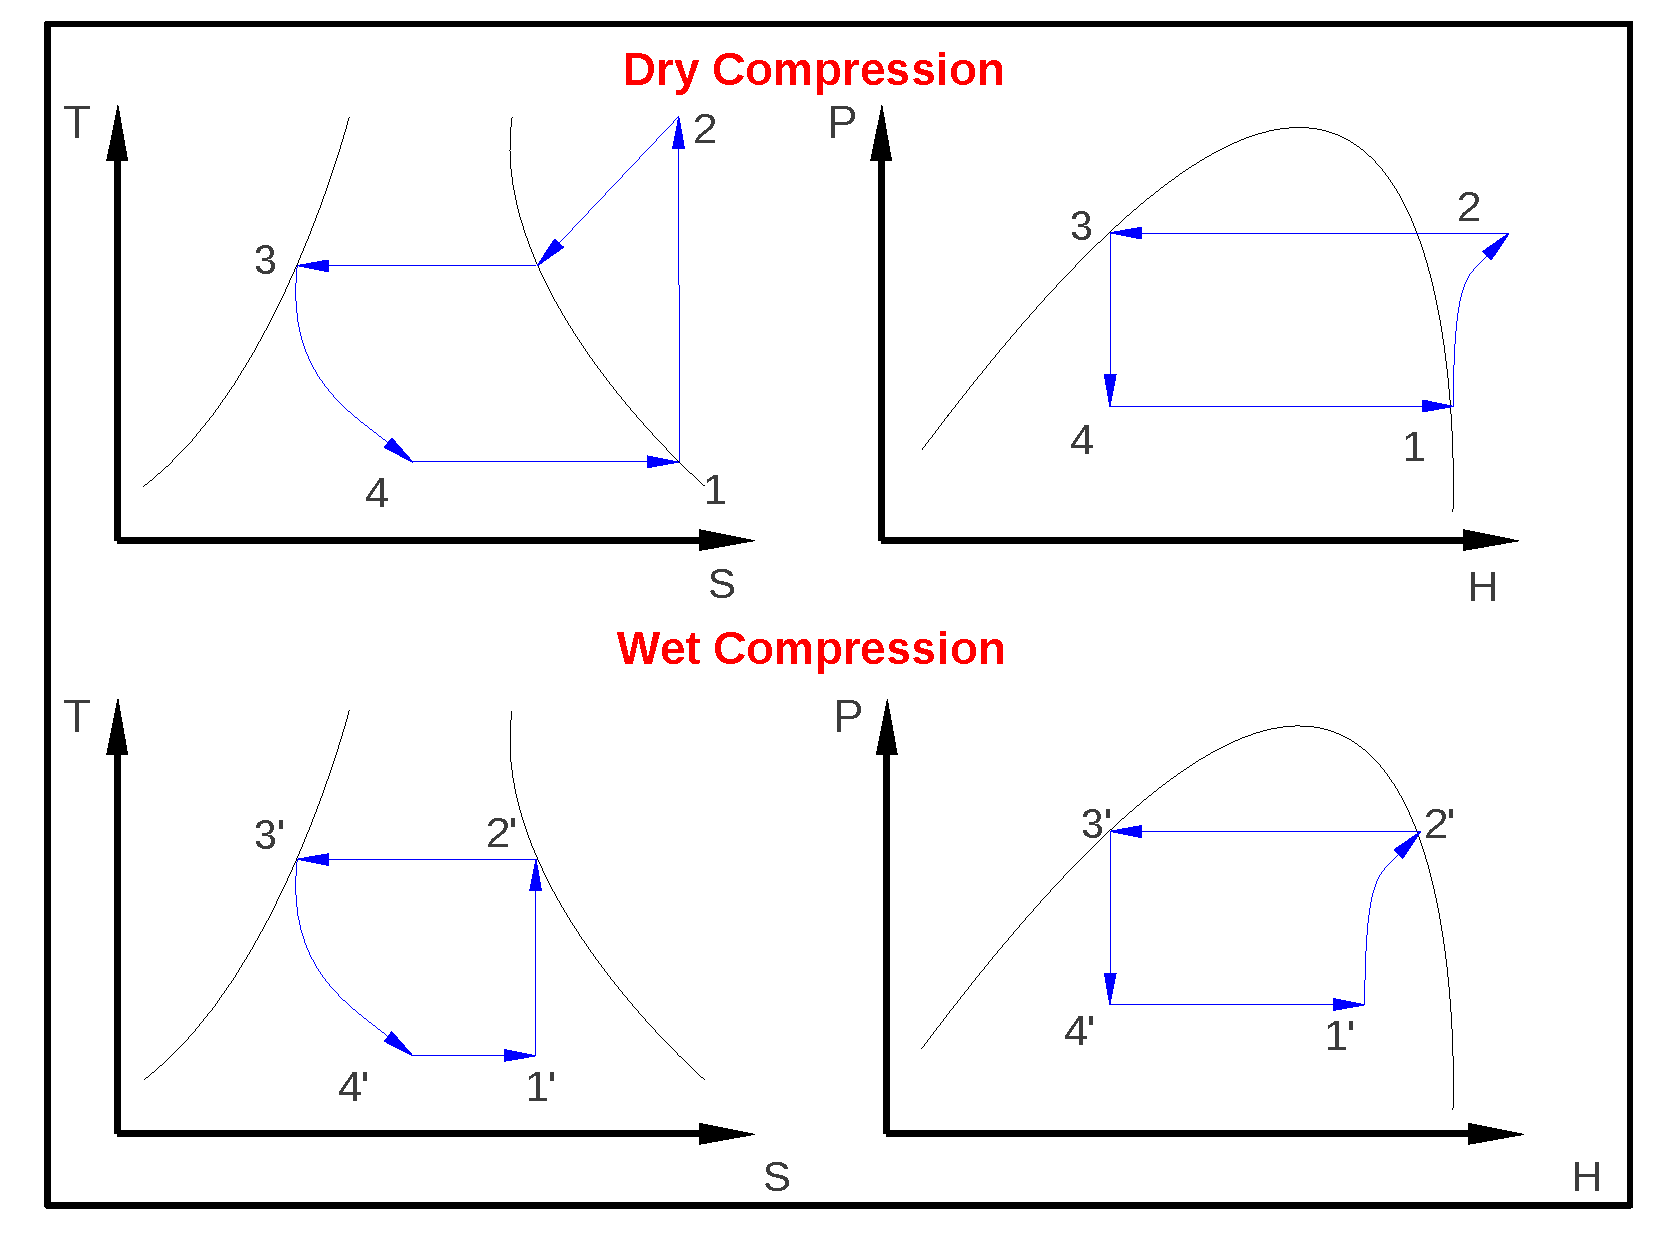
\includegraphics[width=.9\columnwidth]{./Pics/Overview_Refrig13}}}
   \end{column}  

\end{columns}
\end{frame}
 

%%%
%%% Slide
%%%
\begin{frame}
 \frametitle{Thermodynamic Analysis} 
   \begin{figure}%
     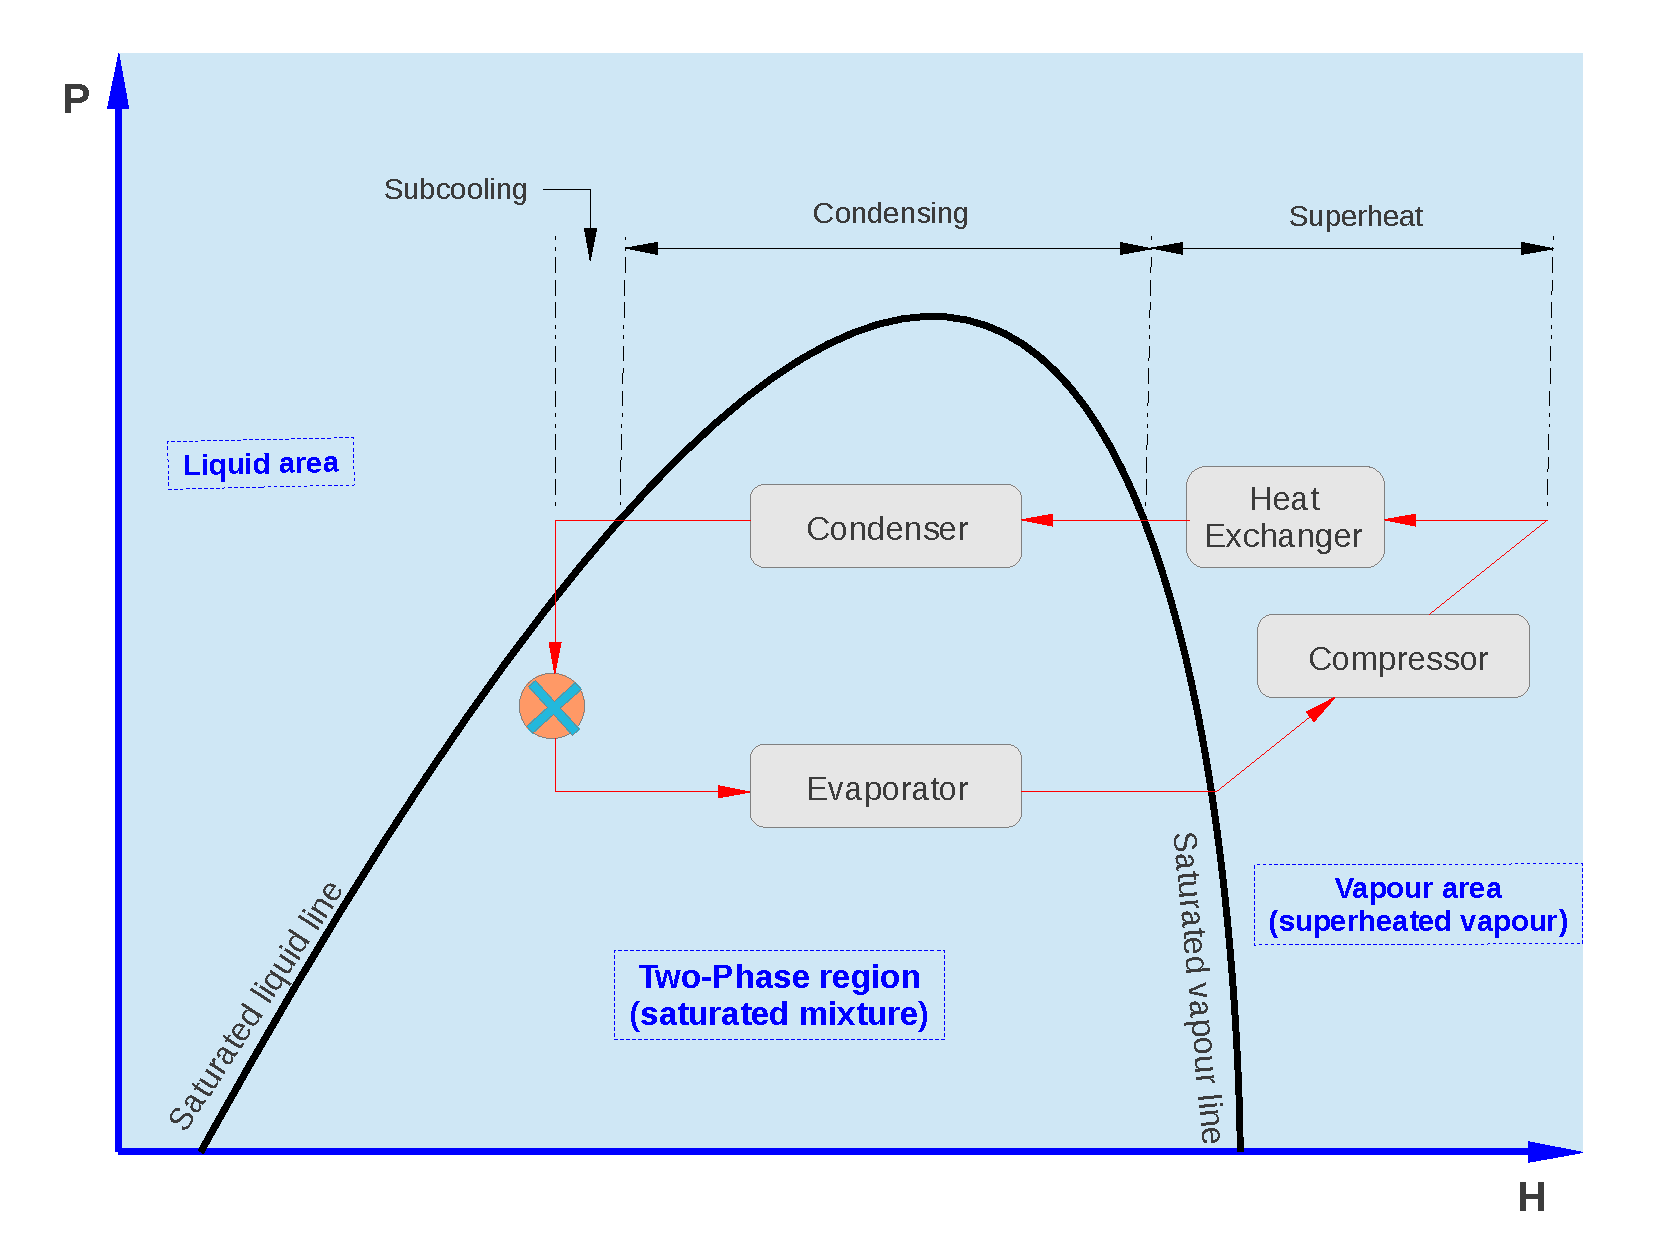
\includegraphics[width=.8\columnwidth]{./Pics/Overview_Refrig19}
   \end{figure}
\end{frame}


%%%
%%% SECTION
%%%
\section{Summary}

%%%
%%% Slides
%%%
\begin{frame}
 \frametitle{Summary}
  After this lecture you should:
 \begin{enumerate}[(a)]
  \item <1-> Identify elements of gas and vapour-compressed refrigeration systems;
  \item <2-> Link the thermo-fluid dynamics learnt in Module 2 with refrigeration cycles;
  \item <3-> Be able to sketch $PH$ and $TS$ diagrams and perform a thermal analysis of the cycles.
 \end{enumerate}
\end{frame}


\end{document}
 

%      \vbox{
%         \hbox{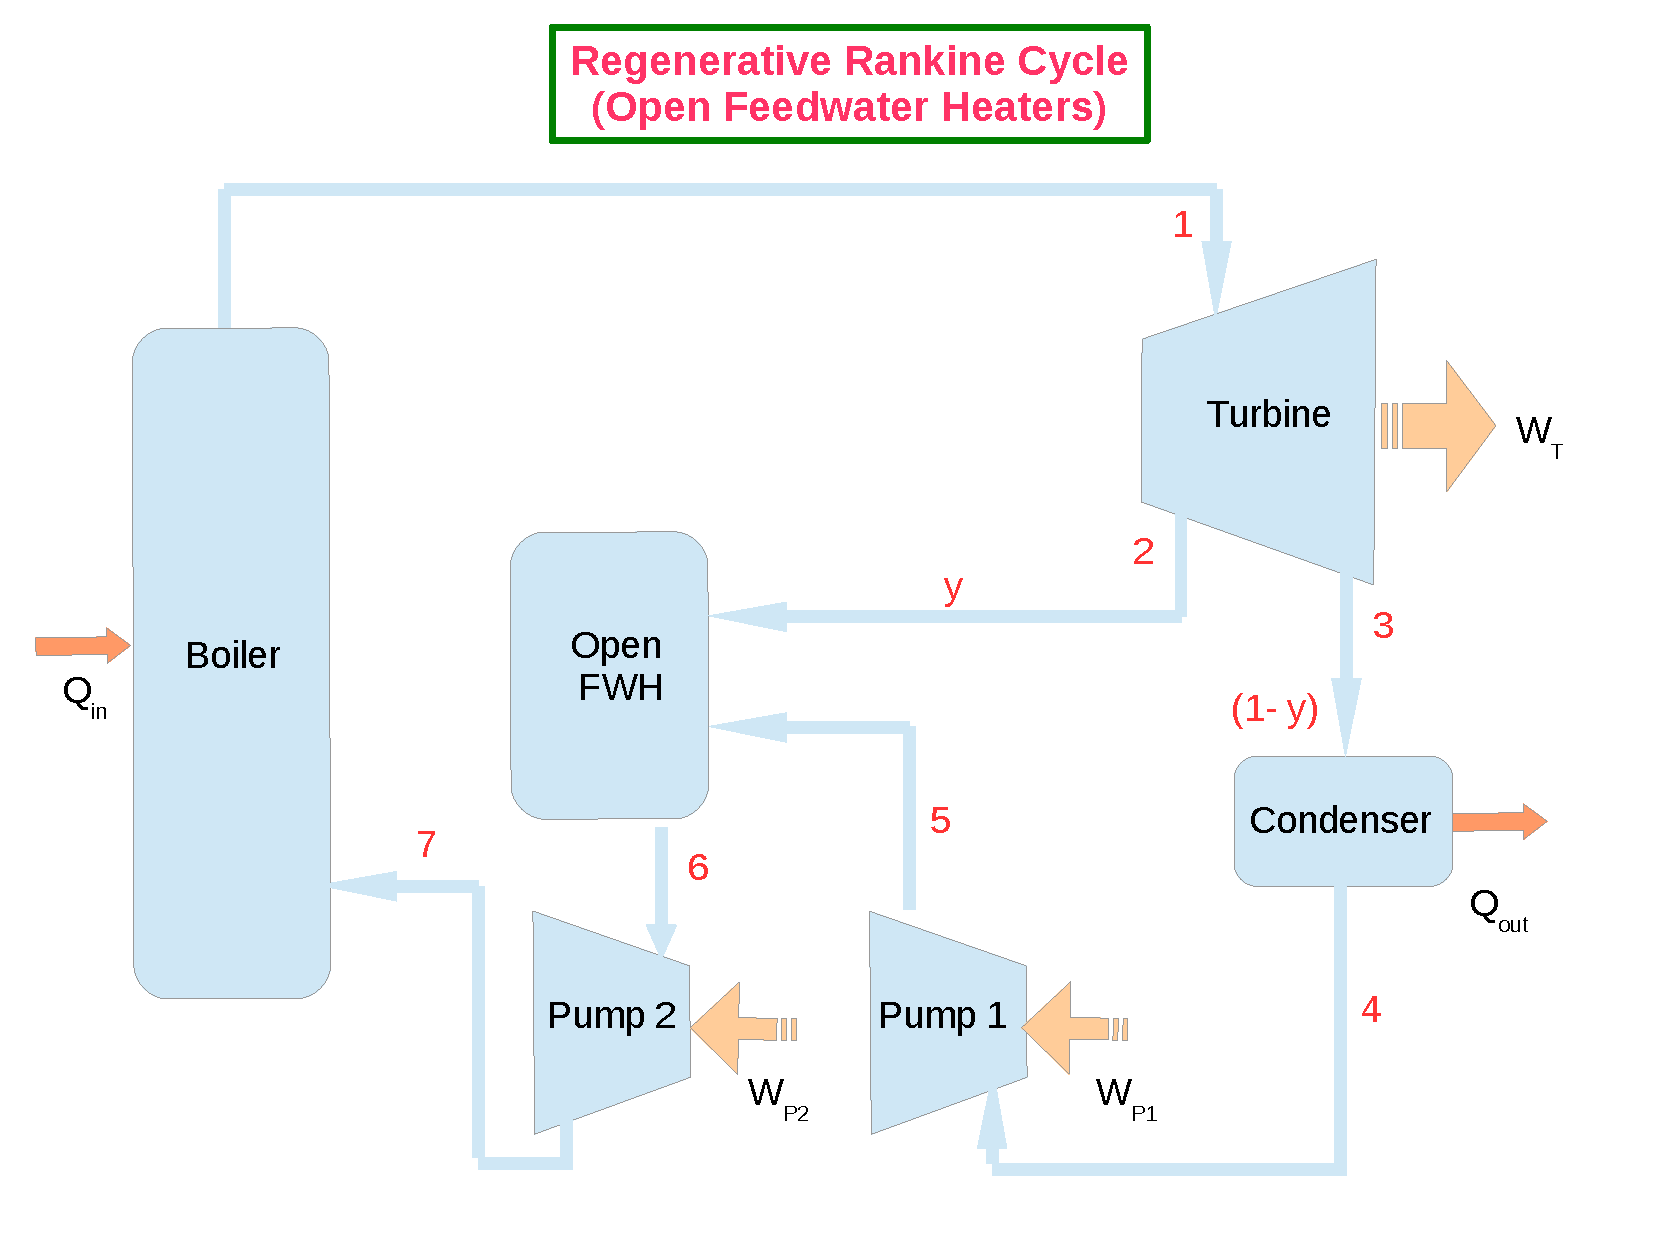
\includegraphics[width=6.cm,clip]{./Pics/RegenerativeOpen_RankineCycle}}
%         \vspace{-0.7cm}
%         \hbox{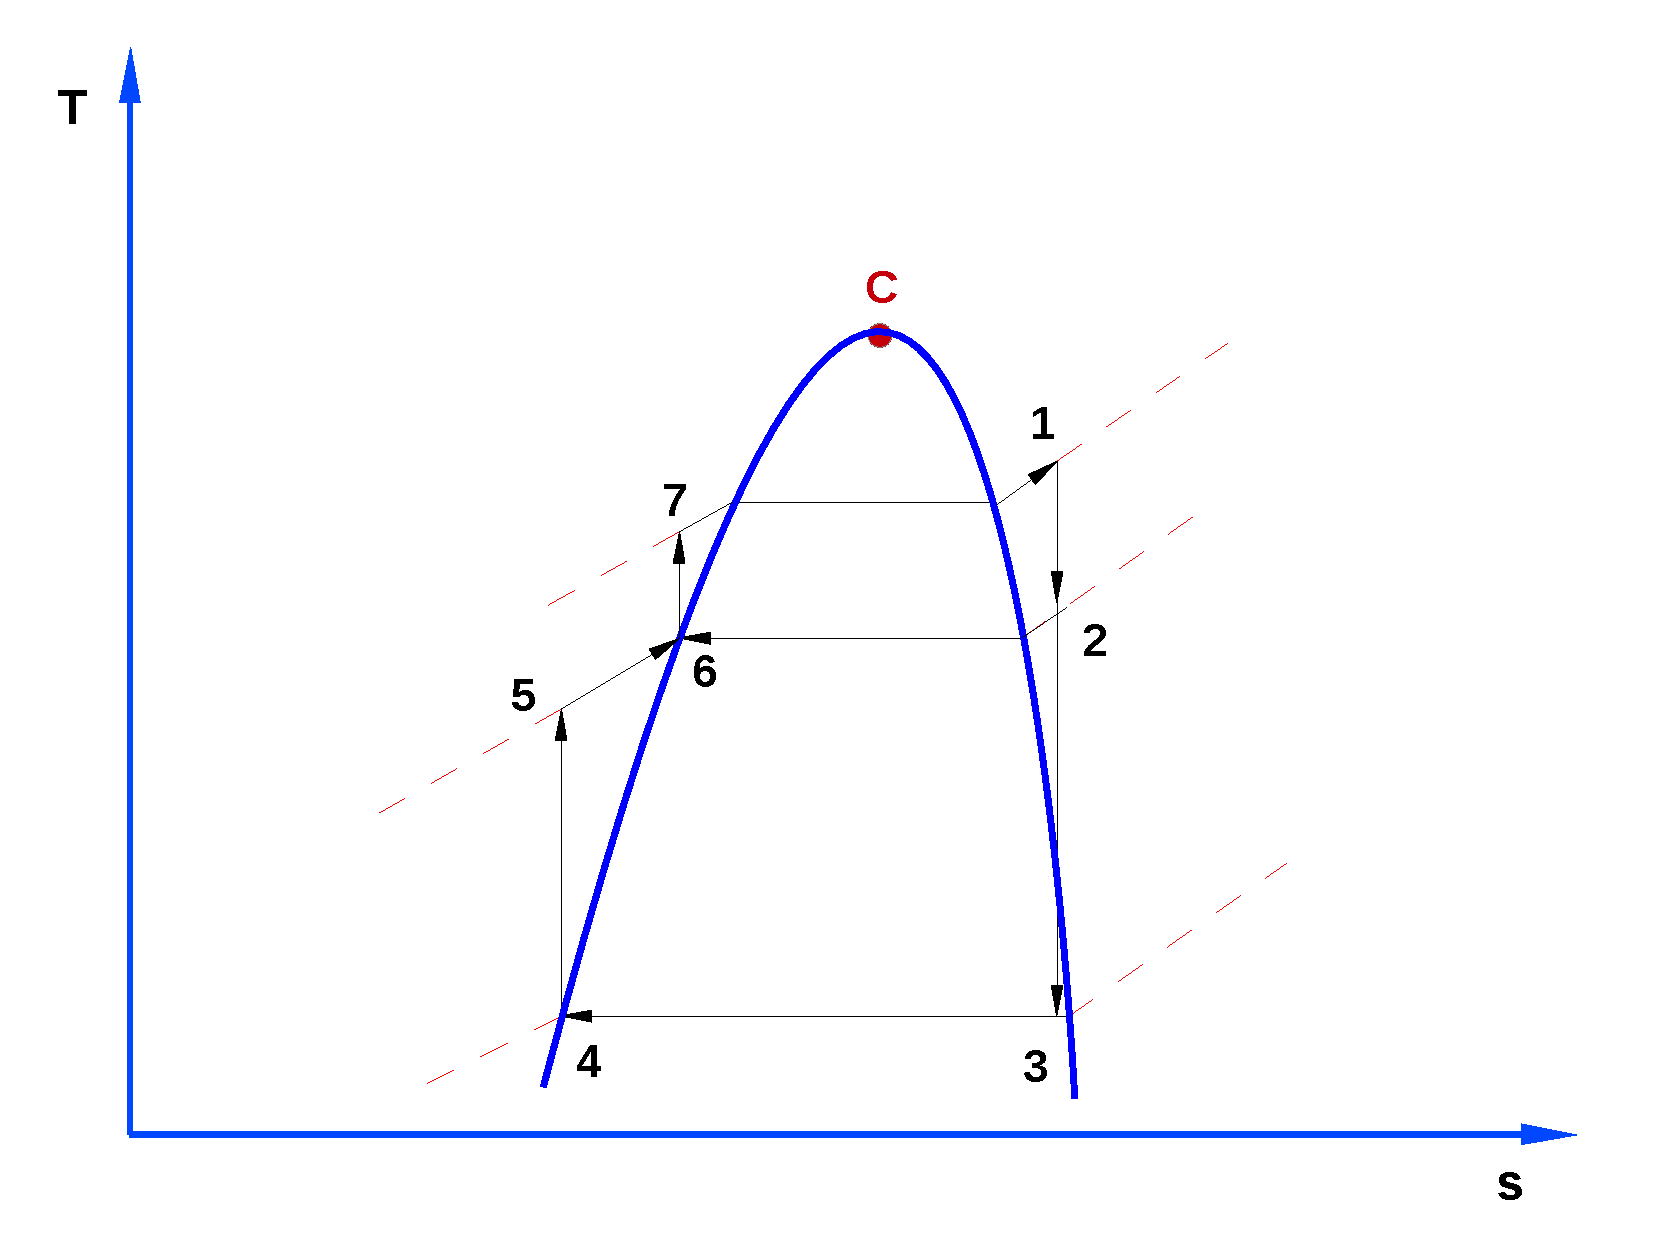
\includegraphics[width=6.cm,clip]{./Pics/RegenerativeOpen_RankineCycle_Diagram}}
%      }  
